\documentclass[11pt, a4paper]{article}
\usepackage[a4paper, margin = 1in]{geometry}
\usepackage{amsmath}
\usepackage{amssymb}
\usepackage{enumitem}
\usepackage{latexsym}
\usepackage{slashed}
\usepackage[compat = 1.1.0]{tikz-feynman}
\usepackage{simpler-wick}

%tikz configuration
\usetikzlibrary{
    external, 
    shapes.misc, 
    decorations.markings,
    decorations.pathreplacing,
    calc
}
\tikzexternalize[
    prefix = tikz-img/,
    system call = {
        lualatex \tikzexternalcheckshellescape -interaction=nonstopmode -jobname="\image" "\texsource" || rm "\image.pdf"
    }
]
\tikzfeynmanset{warn luatex = false}
\tikzset {
    single line/.style = {},
    double line/.style = {double distance = 1pt},
    vertex/.style = {circle, fill, inner sep = 1pt},
    empty/.style = {inner sep = 1pt},
    cross vertex/.style = {cross out, draw, inner sep = 2pt, thick},
    %
    on each segment/.style={
        decorate,
        decoration={
            show path construction,
            moveto code={},
            lineto code={
                \draw [#1]
                (\tikzinputsegmentfirst) -- (\tikzinputsegmentlast);
            },
            curveto code={
                \draw [#1] (\tikzinputsegmentfirst)
                .. controls
                (\tikzinputsegmentsupporta) and (\tikzinputsegmentsupportb)
                ..
                (\tikzinputsegmentlast);
            },
            closepath code={
                \draw [#1]
                (\tikzinputsegmentfirst) -- (\tikzinputsegmentlast);
            },
        },
    },
    mid arrow/.style = {
        postaction = {
            decorate,
            decoration = {
                markings,
                mark = at position .5 with {#1}
            }
        }
    },
    inserted arrow/.pic = {
        \draw [arrows = {-Latex[length = 6pt 0 0]}] (0pt, 0) -- ++(3pt, 0);
    },
    text/.style = {
        insert path = {
            node[
                midway, 
                label = above:#1,
                sloped,
                allow upside down,
                label distance = 1pt
            ]{}
        }
    },
    texti/.style = {
        insert path = {
            node[
                midway, 
                label = below:#1,
                sloped,
                allow upside down,
                label distance = 1pt
            ]{}
        }
    },
    arrowed/.style={
        insert path = {
            pic[midway, sloped, allow upside down]{inserted arrow}
            % node[midway,sloped,allow upside down]{\tikz{ \draw[#1] (-.2pt,0) -- ++(.2 pt,0);}}
        }
    }
}

% math
\newcommand{\dd}{\mathrm{d}}
\newcommand{\df}[2]{\frac{\dd #1}{\dd #2}}
\newcommand{\pd}[2]{\frac{\partial #1}{\partial #2}}
\newcommand{\pdd}[3]{\frac{\partial^2 #1}{\partial #2\partial #3}}
\newcommand{\hodge}{{}^\star}
\newcommand{\lag}{\mathcal{L}}
\newcommand{\cc}{\mathrm{c.c.}}
\newcommand{\hc}{\mathrm{h.c.}}
\newcommand{\tr}{\operatorname{tr}}
\newcommand{\ket}[1]{\left|#1\right\rangle}
\newcommand{\bra}[1]{\left\langle #1\right|}
\newcommand{\inner}[2]{\left\langle #1 \middle| #2 \right\rangle}
\newcommand{\avg}[1]{\left\langle #1 \right\rangle}
\newcommand{\abs}[1]{\left| #1 \right|}
\newcommand{\bigo}{\mathcal{O}}
\newcommand{\ims}{\mathcal{M}}
% counter for problems
\newcounter{problemCounter}[section]
\newcommand{\problem}{\stepcounter{problemCounter}\noindent\textbf{\arabic{section}.\arabic{problemCounter}} \quad}
\newcommand{\solution}{\noindent\textbf{Solutions for \arabic{section}.\arabic{problemCounter}}\quad}
\newenvironment{problembody}
{\begin{enumerate}[label = (\alph*), ref = (\alph*)]}
{\end{enumerate}}

\newcommand{\needverify}{\textsuperscript{[NEED VERIFY]}}

\setlength{\parskip}{6pt}

% chapter 1 has no problem, begin with chapter 2
\setcounter{section}{1}

% equation numbers
\numberwithin{equation}{section}

\numberwithin{problemCounter}{section}

\author{hadroncfy}
\title{Detailed Solutions to Problems in \textit{An Introduction to Quantum Field Theory}}

\begin{document}
\maketitle
\section{Chapter 2}

\setcounter{equation}{66}
\problem Classical electromagnetism (with no sources) follows from the action
\begin{equation}
    S = \int \dd^4 x \left(-\frac{1}{4} F_{\mu\nu} F^{\mu\nu} \right), 
    \qquad \text{where } F_{\mu\nu} = \partial_\mu A_\nu - \partial_\nu A_\mu
\end{equation}
\begin{problembody}
    \item Derive Maxwell's equations as the Eular-Lagrange equations of this action, treating the 
    components $A_\mu$ as the dynamical variables.
    \item Construct the energy-momentum tensor for this theory. Note that the usual procedure does
    not result in a symmetric tensor. To remedy this, we can add to $T^{\mu\nu}$ a term of the form 
    $\partial_\lambda K^{\lambda\mu\nu}$, where $K^{\lambda\mu\nu}$ is antisymmetric in its first two
    indices. Such an object is automatically divergenceless, so
    \begin{equation*}
        \widehat{T}^{\mu\nu} = T^{\mu\nu} + \partial_\lambda K^{\lambda\mu\nu}
    \end{equation*}
    is an equally good energy-momentum tensor with the same globally conserved energy and momentum. Show 
    that this construction with
    \begin{equation*}
        K^{\lambda\mu\nu} = F^{\mu\lambda} A^\nu
    \end{equation*}
    leads to an energy-momentum tensor $\widehat{T}^{\mu\nu}$ that is symmetric and yields the standard
    formulae for the electromagnetic energy and momentum densities
    \begin{equation*}
        \mathcal{E} = \frac{1}{2}(E^2 + B^2); \quad \vec{S} = \vec{E} \times \vec{B}
    \end{equation*}
\end{problembody}

\solution 
\begin{problembody}
    \item The Lagrangian density can be written as
    \begin{equation}\label{equ:cp2:l_den}
        \mathcal{L} = \frac{1}{2} \left(\partial_\mu A_\nu\right)^2 - \frac{1}{2}\partial_\mu A_\nu \partial^\nu A^\mu
    \end{equation}
    substitute \eqref{equ:cp2:l_den} into Eular-Lagrange equation
    \begin{equation}\label{equ:cp2:eular_lagrangian_a}
        \pd{\mathcal{L}}{A_\mu} = \partial_\nu \left(\pd{\mathcal{L}}{(\partial_\nu A_\mu)}\right)
    \end{equation}
    The LHS of \eqref{equ:cp2:eular_lagrangian_a} is zero, while the derivative in the bracket of RHS becomes
    \begin{align*}
        \pd{\mathcal{L}}{(\partial_\nu A^\mu)} 
        & = -\frac{1}{2} F^{\alpha\beta} \left(\delta^\nu_\alpha \delta^\mu_\beta - \delta^\nu_\beta \delta^\mu_\alpha\right)\\
        & = -F^{\nu\mu}
    \end{align*}
    So the equation of motion is
    \begin{equation}\label{equ:cp2:f_maxwell}
        \partial_\nu F^{\nu\mu} = 0
    \end{equation}
    For $\mu = 0$, \eqref{equ:cp2:f_maxwell} yields:
    \begin{equation*}
        \partial_\nu F^{\nu 0} = \partial_i E^i = 0
    \end{equation*}
    which is nothing but $\nabla\cdot\vec{E} = 0$. For $\mu = i$, \eqref{equ:cp2:f_maxwell} becomes
    \begin{align*}
        0 = \partial_\nu F^{\nu i} 
        & = \partial_0 F^{0i} + \partial_j F^{ji}\\
        & = -\pd{E^i}{t} + \epsilon_{ijk}\partial_j B^k
    \end{align*}
    written in vector form, this is just
    \begin{equation*}
        \nabla\times\vec{B} = \pd{\vec{E}}{t}
    \end{equation*}
    \item Consider an infinitesimal translation $x^\mu \to x^\mu + \epsilon^\mu$, the Neother current 
    is 
    \begin{equation}\label{equ:cp2:a_neother}
        T^{\mu\nu} = \pd{\mathcal{L}}{(\partial_\mu A_\lambda)} \partial^\nu A_\lambda - \mathcal{L} g^{\mu\nu}
    \end{equation}
    Substitute \eqref{equ:cp2:eular_lagrangian_a} into \eqref{equ:cp2:a_neother}, we get
    \begin{equation}
        T^{\mu\nu} = -F^{\mu\lambda} \partial^\nu A_\lambda + \frac{1}{4} (F_{\alpha\beta})^2 g^{\mu\nu}
    \end{equation}
    so that
    \begin{align*}
        \widehat{T}^{\mu\nu} 
        & = T^{\mu\nu} + \partial_\lambda F^{\mu\lambda} A^\nu + F^{\mu\lambda} \partial_\lambda A^\nu \\
        & = F^{\mu\lambda} F_\lambda{}^\nu + \frac{1}{4}(F_{\alpha\beta})^2 g^{\mu\nu}
    \end{align*}
    where we have used \eqref{equ:cp2:f_maxwell} in the second step. Now the energy and momentum density 
    can be read as
    \begin{equation*}
        \mathcal{E} = \widehat{T}^{00} = F^{0i}F_i{}^0 + \frac{1}{2}(B^2 - E^2) = \frac{1}{2} (B^2 + E^2)
    \end{equation*}
    \begin{equation*}
        S^i = \widehat{T}^{i0} = F^{0j}F_j{}^i = E^j B^k \epsilon_{jki}
    \end{equation*}
    that is
    \begin{equation*}
        \vec{S} = \vec{E} \times \vec{B}
    \end{equation*}
\end{problembody}

\problem \textbf{The complex scalar field.} Consider the field theory of a complex-valued scalar field obeying 
the klein-Gordon equation. The action of the theory is
\begin{equation}\label{equ:cp2:s_csf}
    S = \int \dd^4x \left(\partial_\mu \phi^\ast \partial^\mu \phi - m^2 \phi^\ast \phi\right)
\end{equation}
It is easiest to analyse this theory by considering $\phi(x)$ and $\phi^\ast(x)$, rather than the real and imaginery
parts of $\phi(x)$, as the basic dynamic varaibles.
\begin{problembody}
    \item Find the conjugate momenta to $\phi(x)$ and $\phi^\ast(x)$ and the canonical commutation relations. Show 
    that the Hamiltonian is
    \begin{equation}\label{equ:cp2:h_csf}
        H = \int \dd^3x \left(\pi^\ast\pi + \nabla\phi^\ast \cdot \nabla\phi + m^2 \phi^\ast\phi\right)
    \end{equation}
    Compute the Heisenburg equation of motion for $\phi(x)$ and show that it is indeed the Klein-Gordon equation.
    
    \item Diagonize \textit{H} by introducing creation and annihilation operators. Show that the theory contains two 
    sets of particles of mass \textit{m}.
    
    \item \label{ex:cp2:charge_1} Rewrite the conserved charge
    \begin{equation}\label{equ:cp2:charge}
        Q = \int \dd^3x \frac{i}{2} \left(\phi^\ast \pi^\ast - \pi\phi\right)
    \end{equation}
    in terms of creation and annihilation operators, and evaluate the charge of the particles of each type.
    
    \item Consider the case of two complex Klein-Gordon fields with the same mass. Label the fields as $\phi_a(x)$,
    where $a = 1,2$. Show that there are now four conserved charges, one given by the generization of part \ref{ex:cp2:charge_1}, 
    and the other three given by
    \begin{equation}\label{equ:cp2:charge_2}
        Q^i = \int \dd^3x \frac{i}{2} (\phi^\ast_a (\sigma^i)_{ab} \pi^\ast_b - \pi_a (\sigma^i)_{ab} \phi_b)
    \end{equation}
    where $\sigma^i$ are the Pauli sigma matrices. Show that these three charges have the commutation relations of 
    angular momentum (\textit{SU}(2)). Generalize these results to the case of \textit{n} identical complex scalar 
    fields.
\end{problembody}

\solution
\begin{problembody}
    \item The conjugate momenta are
    \begin{subequations}\label{equ:cp2:csf_p}
        \begin{align}
            \pi & = \pd{\mathcal{L}}{\dot{\phi}} = \dot{\phi}^\ast \\
            \pi^\ast & = \pd{\mathcal{L}}{\dot{\phi}^\ast} = \dot{\phi}
        \end{align}
    \end{subequations}
    $\pi(x)$ and $\phi(x)$ should satisfy the canonical commutation relations:
    \begin{subequations}\label{equ:cp2:csf_comm}
        \begin{equation}
            [\phi(t, \vec{x}), \phi(t, \vec{y})] = [\phi(t, \vec{x}), \phi^\ast(t, \vec{y})] = 0
        \end{equation}
        \begin{equation}
            [\pi(t, \vec{x}), \pi(t, \vec{y})] = [\pi(t, \vec{x}), \pi^\ast(t, \vec{y})] = 0
        \end{equation}
        \begin{equation}
            [\pi(t, \vec{x}), \phi^\ast(t, \vec{y})] = [\pi^\ast(t, \vec{x}), \phi(t, \vec{y})] = 0
        \end{equation}
        \begin{equation}
            [\phi(t, \vec{x}), \pi(t, \vec{y})] = [\phi^\ast(t, \vec{x}), \pi^\ast(t, \vec{y})] = i\delta^3(\vec{x} - \vec{y})
        \end{equation}
    \end{subequations}
    The Hamiltonian is 
    \begin{align}\label{equ:cp2:csf_hami}
        H & = \int \dd^3x (\pi\phi + \pi^\ast\phi^\ast) - L \nonumber\\
        & = \int \dd^3x \left(\pi^\ast\pi + \nabla\phi^\ast \cdot \nabla\phi + m^2 \phi^\ast\phi\right)
    \end{align}
    Heisenburg equation for $\phi(x)$ is simply
    \begin{equation}\label{equ:cp2:Heisenburg_eq_phi}
        i\dot{\phi} = [\phi, H] = i\pi^\ast
    \end{equation}
    while for $\pi(x)$ is
    \begin{align}\label{equ:cp2:Heisenburg_eq_pi}
        i\dot{\pi}(x) = [\pi(x), H(t)] 
        & = \left[\pi(x), \int \dd^3y (\partial_i \phi^\ast(y) \partial_i\phi(y) + m^2 \phi^\ast(y)\phi(y))\right]\nonumber\\
        & = \left[\pi(x), \int \dd^3y \phi(y)(-\nabla^2 + m^2)\phi^\ast(y)\right]\nonumber\\
        & = i(\nabla^2 - m^2) \phi^\ast(x)
    \end{align}
    where $x^0 = y^0 = t$, and we have integrated by parts at second step. Combining \eqref{equ:cp2:Heisenburg_eq_phi} 
    and \eqref{equ:cp2:Heisenburg_eq_pi} we obtain the equation of motion
    \begin{equation}\label{equ:cp2:csf_equation_of_motion}
        \ddot{\phi} = \dot{\pi}^\ast = (\nabla^2 - m^2)\phi
    \end{equation}
    which is nothing but the Klein-Gordon equation $(\Box + m^2)\phi = 0$.

    \item $\phi(x)$ can be expanded in terms of plain waves as
    \begin{equation}\label{equ:cp2:phi_expand}
        \phi(x) = \sum_k \left(a_k \varphi_k + b^\dagger_k \varphi^\ast_k \right)
    \end{equation}
    where $a_k$ and $b_k$ are annihilation operators, and the plain wave function $\varphi_k(x)$ is 
    \begin{equation}\label{equ:cp2:plain_w}
        \varphi_k(t, \vec{x}) = \frac{1}{\sqrt{2V\omega_k}}e^{-i\omega_kt + i\vec{k}\cdot\vec{x}}
    \end{equation}
    where $\omega_k = \sqrt{k^2 + m^2}$. Define inner product $\langle\cdot,\cdot\rangle$ as follow
    \begin{equation}\label{equ:cp2:inner_prod}
        \langle f, g \rangle \equiv i \int \dd^3x (f^\ast\dot{g} - \dot{f}^\ast g)
    \end{equation}
    so the inner products of the plain wave functions are
    \begin{align*}
        \langle \varphi_k, \varphi_{k'} \rangle & = \delta_{kk'}\\
        \langle \varphi^\ast_k, \varphi^\ast_{k'} \rangle & = -\delta_{kk'}\\
        \langle \varphi_k, \varphi^\ast_{k'} \rangle & = 0
    \end{align*}
    Notice that the second slot of the inner product is linear, while the first slot is antilinear. 
    Then the operators $a_k$ and $b_k$ can be expressed as
    \begin{subequations}\label{equ:cp2:csf_optr_a_b}
        \begin{align}
            a_k & = \langle \varphi_k, \phi \rangle = \int \dd^3x \, \varphi^\ast_k \left(\omega_k\phi + i\pi^\ast\right)\\
            b_k & = -\langle \varphi^\ast_k, \phi \rangle^\ast = \int \dd^3x \, \varphi^\ast_k \left(\omega_k\phi^\ast + i\pi\right)
        \end{align}
    \end{subequations}
    using \eqref{equ:cp2:csf_comm}, we get the commutation relations for operators $a_k$ and $b_k$:
    \begin{subequations}\label{equ:cp2:csf_a_b_com}
        \begin{equation}
            [a_k,a_{k'}] = [b_k, b_{k'}] = 0
        \end{equation}
        \begin{equation}
            [a_k,b_{k'}] = [a_k, b_{k'}^\dagger] = 0
        \end{equation}
        \begin{equation}
            [a_k, a_{k'}^\dagger] = [b_k, b_{k'}^\dagger] = \delta_{kk'}
        \end{equation}
    \end{subequations}
    substitute \eqref{equ:cp2:phi_expand} into \eqref{equ:cp2:csf_hami}, and using \eqref{equ:cp2:csf_a_b_com}, we get the 
    Hamiltonian written in terms of creation and annihilation operators
    \begin{align}\label{equ:cp2:csf_hami_diag}
        H & = \sum_{k, k'}\left(\omega_k\omega_{k'} + \vec{k}\cdot\vec{k}' + m^2\right)
        \int \dd^3x \, \left(a^\dagger_k\varphi^\ast_k - b_k\varphi_k\right)
        \left(a_{k'}\varphi_{k'} - b^\dagger_{k'}\varphi^\ast_{k'}\right)\nonumber\\
        & = \sum_{k, k'}\left(\omega_k\omega_{k'} + \vec{k}\cdot\vec{k}' + m^2\right)
        \int \dd^3x \, \left(a^\dagger_k a_{k'} \varphi^\ast_k \varphi_{k'} + b_k b^\dagger_{k'} \varphi_k \varphi^\ast_{k'}\right)\nonumber\\
        & = \sum_k \omega_k \left(a^\dagger_k a_k + b^\dagger_k b_k + 1\right)
    \end{align}
    so this theory contains two sets of particles with mass \textit{m}, created by $a^\dagger_k$ and $b^\dagger_k$, respectively.
    Notice that the energy of ground state is infinity, but it's irrelavent, since we only concern energy differences.

    \item Substitute \eqref{equ:cp2:phi_expand} into \eqref{equ:cp2:charge}, we get
    \begin{align}\label{equ:cp2:charge_diag}
        Q & = \frac{i}{2} \left[\sum_{k, k'} (-i\omega_{k'})
        \int \dd^3x \, \left(a^\dagger_k\varphi^\ast_k + b_k\varphi_k\right)
        \left(a_{k'} \varphi_{k'} - b^\dagger_{k'}\varphi^\ast_{k'}\right) - h.c.\right]\nonumber\\
        & = \frac{i}{2} \left[-\frac{i}{2} \sum_k \left(a^\dagger_k a_k - b_k b^\dagger_k\right) - h.c.\right]\nonumber\\
        & = \frac{1}{2} \sum_k \left(a^\dagger_k a_k - b^\dagger_k b_k\right)
    \end{align}
    Where we have ignored an infinite constant in the last step. So the two sets of particles created by $a^\dagger_k$ and $b^\dagger_k$ have charges
    $\frac{1}{2}$ and $-\frac{1}{2}$, respectively.

    \item We first consider the general case of \textit{n} fields, the case of two fields can be obtained by setting $n = 2$. Let the \textit{n} fields to be 
    $\phi_a(x)$, where $a = 1, 2, \cdots, n$, define
    \begin{equation*}
        \phi = \begin{pmatrix}
            \phi_1\\
            \phi_2\\
            \vdots\\
            \phi_n
        \end{pmatrix},
        \pi = \left(\pi_1, \pi_2, \cdots, \pi_n\right)
    \end{equation*}
    The Lagrangian can be written as 
    \begin{equation}\label{equ:cp2:csf_nf_lag}
        \mathcal{L} = \partial_\mu \phi^\dagger \partial^\mu \phi - m^2 \phi^\dagger \phi
    \end{equation}
    It is invariant under global transformation
    \begin{equation*}
        \phi \to A \phi
    \end{equation*}
    where $A \in U(n)$ is an $n \times n$ matrix. Since $U(n) = SU(n) \otimes U(1)$, the infinitesimal transformation can be expressed as
    \begin{equation*}
        \phi \to (I - i\alpha - i t^i \theta^i)\phi
    \end{equation*}
    where $\alpha$ and $\theta^i$ are infinitesimal parameters, correspond to $U(1)$ and $SU(n)$ respectively, 
    matrices $t^i$ are generators of $SU(n)$, $i = 1, 2, \cdots, (n^2 - 1)$. By Neother's theorem, 
    $\alpha$ yields one conserved charge:
    \begin{align*}
        q & = \frac{1}{\alpha}\int \dd^3x \, \left(\pd{\mathcal{L}}{(\partial_0\phi)}(-i\alpha\phi) + (i\alpha\phi^\dagger)\pd{\mathcal{L}}{(\partial_0\phi^\dagger)}\right)\\
        & = \int \dd^3x \, \left(\phi^\dagger \pi^\dagger - \pi\phi\right)
    \end{align*}
    the $SU(n)$ transformation yields $n^2 - 1$ charges:
    \begin{align*}
        Q^i & = \frac{1}{\theta^i}\int \dd^3x \, \left(\pd{\mathcal{L}}{(\partial_0\phi)} (-it^i\phi) + (it^i \phi^\dagger)\pd{\mathcal{L}}{(\partial_0\phi)} \right)\\
        & = \int \dd^3x \, \left(\phi^\dagger t^i \pi^\dagger - \pi t^i \phi\right)
    \end{align*}
    There are totally $n^2$ charges. In the case $n = 2$, there are 4 charges, and $t^i$ become the Pauli sigma matrices.
\end{problembody}

\problem Evaluate the function
\begin{equation*}
    \langle 0 | \phi(x) \phi(y) |0 \rangle = D(x - y) = \int \frac{\dd^3p}{(2\pi)^3} \frac{1}{2E_\mathbf{p}} e^{-ip \cdot (x - y)}
\end{equation*}
for $(x - y)$ spacelike so that $(x - y)^2 = -r^2$, explicitly in terms of Bessel functions.

\solution
\begin{align*}
    D(x - y) & = \int \frac{\dd^3p}{(2\pi)^3} \frac{1}{2E_{\mathbf{p}}} e^{i\vec{p}\cdot(\vec{x} - \vec{y})}\\
    & = \frac{1}{4\pi^2} \int_0^{+\infty} \frac{p^2}{2E_{\mathbf{p}}} \dd p \int_{-1}^1 \dd (\cos\theta) e^{ipr\cos\theta}\\
    & = \frac{1}{8\pi^2ir} \int_0^{+\infty} \frac{p}{E_{\mathbf{p}}} \left(e^{ipr} - e^{-ipr}\right)\\
    & = \frac{1}{8\pi^2ir} \int_{-\infty}^{+\infty} \frac{p}{\sqrt{p^2 + m^2}} e^{ipr} \dd p\\
    & = \frac{1}{8\pi^2ir} \left[\int_{+im}^{+i\infty} \frac{p}{i\sqrt{-p^2 - m^2}} e^{ipr} \dd p + \int_{+i\infty}^{im} \frac{p}{-i\sqrt{-p^2 - m^2}} e^{ipr} \dd p \right]\\
    & = \frac{1}{4\pi^2r} \int_m^{+\infty} \frac{x}{\sqrt{x^2 - m^2}} e^{-rx} \dd x\\
    & = \frac{1}{4\pi^2r} \int_0^{+\infty} e^{-r\sqrt{p^2 + m^2}} \dd p\\
    & = \frac{m}{4\pi^2r} \int_0^{+\infty} e^{-mr\cosh t} \cosh t \dd t\\
    & = \frac{m}{4\pi^2r} K_1(mr)
\end{align*}
where 
\begin{equation*}
    K_\alpha(x) = \int_0^{+\infty} e^{-x\cosh t} \cosh{\alpha t} \dd t, \quad Re(x) > 0
\end{equation*}
is the modified Bessel function.
\section{Chapter 3}

\setcounter{equation}{150}
\problem \textbf{Lorentz group.} Recall from Eq. (3.17) the Lorentz commutation relations,
\begin{equation*}
    [J^{\mu\nu}, J^{\rho\sigma}] = i(g^{\nu\rho}J^{\mu\sigma} - g^{\mu\rho}J^{\nu\sigma} - g^{\nu\sigma}J^{\mu\rho} + g^{\mu\sigma}J^{\nu\rho})
\end{equation*}
\begin{problembody}
    \item \label{ex:cp3:lor_gen_com} 
    Define the generators of rotations and boosts as
    \begin{equation*}
        L^i = \frac{1}{2}\epsilon^{ijk} J^{jk}, \quad K^i = J^{0i}
    \end{equation*}
    where $i, j, k = 1, 2, 3$. An infinitesimal Lorentz transformation can then be written
    \begin{equation}\label{equ:cp2:infsm_lor_trans}
        \Phi \to \left(1 - i\vec{\theta}\cdot\vec{L} - i\vec{\beta}\cdot\vec{K}\right)\Phi
    \end{equation}
    Write the commutation relations of these operators explicitly. (For example, $[L^i, L^j] = i\epsilon^{ijk}L^k$)
    Show that the combinations 
    \begin{equation*}
        \vec{J}_{+} = \frac{1}{2} \left(\vec{L} + i\vec{K}\right) \quad \text{and} 
        \quad \vec{J}_{-} = \frac{1}{2} \left(\vec{L} - i\vec{K}\right)
    \end{equation*} 
    commute with one another and separately satisfy the commutation relations of angular momentum.

    \item The finite-dimensional representations of the rotation group correspond precisely to the allowed values for 
    angular momentum: integers or half-integers. The result of part \ref{ex:cp3:lor_gen_com} implies that all finite-dimensional
    representations of the Lorentz group correspond to pairs of integers or half integers, $(j_+, j_-)$, corresponding to pairs 
    of representations of the rotation group. Using the fact that $\vec{J} = \vec{\sigma} / 2$ in the spin-laws of the 2-component
    objects transforming according to the $(\frac{1}{2}, 0)$ and $(0, \frac{1}{2})$ representations of the Lorentz group. Show 
    that these correspond precisely to the transformations of $\psi_L$ and $\psi_R$ given in (3.27).

    \item The identity $\vec{\sigma}^T = -\sigma^2 \vec{\sigma}\sigma^2$ allows us to rewrite the $\psi_L$ transformation in the 
    unitarily equivalent form
    \begin{equation*}
        \psi' \to \psi' \left(1 + i\vec{\theta}\cdot\frac{\vec{\sigma}}{2} + \vec{\beta}\cdot\frac{\vec{\sigma}}{2}\right),
    \end{equation*}
    where $\psi' = \psi_L^T \sigma^2$. Using this law, we can represent the object that transforms as $(\frac{1}{2}, \frac{1}{2})$
    as a $2 \times 2$ matrix that has the $\psi_R$ transformation law on the left and, simutaneously, the transposed $\psi_L$ transformation
    on the right. Parametrize this matrix as
    \begin{equation*}
        \begin{pmatrix}
            V^0 + V^3  & V^1 - iV^2 \\
            V^1 + iV^2 & V^0 - V^3
        \end{pmatrix}.
    \end{equation*}
    Show that the object $V^\mu$ transformations as a 4-vector.
\end{problembody}

\solution
\begin{problembody}
    \item There are 3 sets of commutators. Commutators of the rotation generators are
    \begin{align*}
        [L^i, L^j] & = \frac{1}{4} \epsilon^{ikl} \epsilon^{jmn} [J^{kl}, J^{mn}]\\
        & = \frac{i}{4} \epsilon^{ikl} \epsilon^{jmn} \left(g^{lm}J^{kn} + g^{kn}J^{lm} - g^{km}J^{ln} - g^{ln}J^{km}\right)\\
        & = \frac{i}{4} \left(-\epsilon^{ikm}\epsilon^{jmn}J^{kn} - \epsilon^{ikl}\epsilon^{jmk}J^{lm} 
        + \epsilon^{ikl}\epsilon^{jkn}J^{ln} + \epsilon^{ikl}\epsilon^{jml}J^{km}\right)\\
        & = i J^{ij}\\
        & = i \epsilon^{ijk} L^k
    \end{align*}
    Commutators of the boost generators are
    \begin{align*}
        [K^i, K^j] & = [J^{0i}, J^{0j}]\\
        & = i\left(g^{i0}J^{0j} + g^{0j}J^{i0} - g^{00}J^{ij} - g^{ij}J^{00}\right)\\
        & = -iJ^{ij}\\
        & = -i \epsilon^{ijk} L^k
    \end{align*}
    Commutators between rotation generators and boost generators are
    \begin{align*}
        [L^i, K^j] & = \frac{1}{2} \epsilon^{ikl} [J^{kl}, J^{0j}]\\
        & = \frac{i}{2} \epsilon^{ikl} \left(g^{l0}J^{kj} + g^{kj}J^{l0} - g^{k0}J^{lj} - g^{lj}J^{k0}\right)\\
        & = i\epsilon^{ijk} J^{0k}\\
        & = i\epsilon^{ijk} K^j
    \end{align*}
    And the commutation relations of $\vec{J}_\pm$ are
    \begin{align*}
        [J^i_\pm, J^j_\pm] & = \frac{1}{4}[L^i \pm iK^i, L^j \pm iK^j]\\
        & = \frac{1}{4} \left(i\epsilon^{ijk}L^k \mp 2i\epsilon^{ijk}K^k + i\epsilon^{ijk}L^k\right)\\
        & = \frac{i}{2} \epsilon^{ijk} \left(L^k \pm iK^k\right)\\
        & = i\epsilon^{ijk} J^k_\pm
    \end{align*}
    that is, $\vec{J}_\pm$ satisfy the commutation relations of angular momentum. Further more, the commutators between 
    $\vec{J}_+$ and $\vec{J}_-$ are
    \begin{align*}
        [J^i_+, J^j_-] & = \frac{1}{4} [L^i + iK^i, L^j - iK^j]\\
        & = \frac{1}{4} \left(i\epsilon^{ijk}L^k + \epsilon^{ijk}K^k - \epsilon^{ijk}K^k -i\epsilon^{ijk}L^k\right)\\
        & = 0
    \end{align*}
    So $\vec{J}_+$ and $\vec{J}_-$ commutes with each other.

    \item The infinitesimal transformation \eqref{equ:cp2:infsm_lor_trans} can now be written, in terms of $\vec{J}_\pm$, as
    \begin{equation}\label{equ:cp3:lor_uni_trans}
        \Phi \to \left[1 - i\left(\vec{\theta} - i\vec{\beta}\right)\cdot\vec{J}_+ - i\left(\vec{\theta} + i\vec{\beta}\right)\cdot\vec{J}_-\right] \Phi
    \end{equation}
    for $(\frac{1}{2}, 0)$, make substitution
    \begin{equation*}
        \vec{J}_+ \to \frac{\vec{\sigma}}{2}, \quad \vec{J}_- \to \vec{0}
    \end{equation*}
    so that the transformation is
    \begin{equation}\label{equ:cp3:spinor_trans_L}
        \psi \to \left(1 - i\vec{\theta}\cdot\frac{\vec{\sigma}}{2} - \vec{\beta}\cdot\frac{\vec{\sigma}}{2}\right)\psi
    \end{equation}
    which is the same as the transformation of $\psi_L$ in (3.37). Similarly, for $(0, \frac{1}{2})$, the transformation is
    \begin{equation*}
        \psi \to \left(1 - i\vec{\theta}\cdot\frac{\vec{\sigma}}{2} + \vec{\beta}\cdot\frac{\vec{\sigma}}{2}\right) \psi
    \end{equation*}
    which is the transformation of $\psi_R$.

    \item The matrix can be written as $V^0 + \vec{\sigma}\cdot\vec{V}$. Let $\vec{\alpha} = \vec{\theta} - i\vec{\beta}$,
    Then the (infinitesimal) transformation for the matrix is
    \begin{align*}
        V^0 + \vec{\sigma}\cdot\vec{V} & \to 
        \left(1 - i\vec{\alpha}^\ast\cdot\frac{\vec{\sigma}}{2}\right)
        \left(V^0 + \vec{\sigma}\cdot\vec{V}\right)
        \left(1 + i\vec{\alpha}\cdot\frac{\vec{\sigma}}{2}\right)\\
        & = \left(1 + \vec{\beta}\cdot\vec{\sigma}\right) V^0 + \vec{\sigma}\cdot\vec{V} + \vec{\beta}\cdot\vec{V} + \left(\vec{\theta}\times\vec{V}\right)\cdot\vec{\sigma}\\
        & = V^0 + \vec{\beta}\cdot\vec{V} + \left(\vec{V} + \vec{\beta}V^0 + \vec{\theta}\times\vec{V}\right)\cdot\vec{\sigma}
    \end{align*}
    Thus, the infinitesimal transformation of $V^\mu$ is
    \begin{subequations}\label{equ:cp3:v_trans}
        \begin{align}
            V^0 & \to V^0 + \vec{\beta}\cdot\vec{V}\\
            \vec{V} & \to \vec{V} + \vec{\beta}V^0 + \vec{\theta}\times\vec{V}
        \end{align}
    \end{subequations}
    This is exactly the transformation law for 4-vectors. To make it more obvious, let
    \begin{subequations}\label{equ:cp3:omega_def}
        \begin{align}
            \omega_{0i} & = \beta_i \\
            \omega_{ij} & = \epsilon_{ijk} \theta^k
        \end{align}
    \end{subequations}
    So that \eqref{equ:cp3:v_trans} can be written in 4-vector form as
    \begin{equation*}
        V^\mu \to V^\mu + \omega^\mu{}_\nu V^\nu
    \end{equation*}
    Which is the same as (3.19) by setting $(\mathcal{J}^{\mu\nu})_{\alpha\beta} = 2i \delta^{[\mu}_\alpha \delta^{\nu]}_\beta$.
\end{problembody}

\problem Derive the \textit{Gordon identity},
\begin{equation}\label{equ:cp3:gordon_identity}
    \bar{u}(p')\gamma^\mu u(p) = \bar{u}(p') \left[\frac{p'^{\mu} + p^\mu}{2m} + \frac{i\sigma^{\mu\nu}q_\nu}{2m}\right] u(p)
\end{equation}
where $q = (p' - p)$. We will put this formula to use in Chapter 6.

\solution
\begin{align*}
    \bar{u}(p')\frac{i\sigma^{\mu\nu}q_\nu}{2m} u(p) 
    & = -\frac{1}{4m} \bar{u}(p') \left[\gamma^\mu(\slashed{p}' - \slashed{p}) - (\slashed{p}' - \slashed p) \gamma^\mu \right] u(p)\\
    & = -\frac{1}{4m} \bar{u}(p') \left[-2\slashed{p}'\gamma^\mu - 2\gamma^\mu\slashed{p} + 2(p'^\mu + p^\mu) \right] u(p)\\
    & = \bar{u}(p')\gamma^\mu u(p) - \bar{u}(p')\frac{p'^\mu + p^\mu}{2m}u(p)
\end{align*}
Moving the second term of RHS to LHS, we obtain \eqref{equ:cp3:gordon_identity}.

\problem \textbf{Spinor products.} (This problem, together with Problems 5.3 and 5.6, introduces an efficient computational method for
processes involving massless particles.) Let $k_0^\mu$, $k_1^\mu$ be fixed 4-vectors satisfying $k_0^2 = 0, k_1^2 = -1, k_0\cdot k_1 = 0$.
Define basic spinors in the following way: Let $u_{L0}$ be the left-handed spinor for a fermion with momentum $k_0$. Let $u_{R0} = \slashed{k}_1 u_{L0}$.
Then, for any $p$ such that $p$ is lightlike ($p^2 = 0$), define
\begin{equation*}
    u_L(p) = \frac{1}{\sqrt{2p\cdot k_0}} \slashed{p} u_{R0}, \qquad u_R(p) = \frac{1}{\sqrt{2p\cdot k_0}}  \slashed{p} u_{L0}
\end{equation*}
This set of convensions define defines the phase of spinors unambiguously (except when $p$ is paralle to $k_0$).
\begin{problembody}
    \item Show that $\slashed{k}_0 u_{R0} = 0$. Show that, for any lightlike $p$, $\slashed{p}u_L(p) = \slashed{p}u_R(p) = 0$.
    \item \label{ex:cp3:sp_choices} For choices $k_0 = (E, 0, 0, -E)$, $k_1 = (0, 1, 0, 0)$, construct $u_{L0}$, $u_{R0}$, $u_L(p)$, and $u_R(p)$ explicitly.
    \item Define the \textit{spinor products} $s(p_1, p_2)$ and $t(p_1, p_2)$, for $p_1$, $p_2$ lightlike, by
    \begin{equation*}
        s(p_1, p_2) = \bar{u}_R(p_1) u_L(p_2), \qquad t(p_1, p_2) = \bar{u}_L(p_1) u_R(p_2)
    \end{equation*}
    Using the explicit forms for the $u_\lambda$ given in part \ref{ex:cp3:sp_choices}, compute the spinor products explicitly and show that
    $t(p_1, p_2) = (s(p_2, p_1))^\ast$ and $s(p_1, p_2) = -s(p_2, p_1)$. In addition, show that
    \begin{equation*}
        \left| s(p_1, p_2) \right|^2 = 2p_1 \cdot p_2
    \end{equation*}
    Thus the spinor products are the square roots of 4-vector dot products.
\end{problembody}

\solution
\begin{problembody}
    \item Since $\slashed{k}_0 u_{L0} = 0$, so that
    \begin{equation*}
        \slashed{k}_0 u_{R0} = \slashed{k}_0 \slashed{k}_1 u_{L0} = \left(2k_0 \cdot k_1 - \slashed{k}_1 \slashed{k}_0\right) u_{L0} = 0
    \end{equation*}
    The next two equations are obvious, since $\slashed{p}\slashed{p} = p^2 = 0$.

    \item A left-handed massless particle with the given momentum $k_0$ has $\xi = (1 \, 0)^T$. Using (3.50) we get
    \begin{equation*}
        u_{L0}(k_0) = \sqrt{2E} \begin{pmatrix}
            1\\ 0\\ 0\\ 0
        \end{pmatrix}
    \end{equation*}
    and
    \begin{equation*}
        u_{R0}(k_0) = \slashed{k}_1 u_{L0}(k_0) = \begin{pmatrix}
            0 & -\sigma_x \\
            \sigma_x & 0
        \end{pmatrix} u_{L0}(k_0) = \sqrt{2E}\begin{pmatrix}
            0 \\ 0 \\ 0 \\ 1
        \end{pmatrix}
    \end{equation*}
    \begin{equation*}
        u_L(p) = \frac{1}{\sqrt{E_p + p_z}} \begin{pmatrix}
            0 & E_p - \vec{p}\cdot\vec{\sigma} \\
            E_p + \vec{p}\cdot\vec{\sigma} & 0
        \end{pmatrix} \begin{pmatrix}
            0 \\
            \begin{pmatrix}
                0 \\ 1
            \end{pmatrix}
        \end{pmatrix} = \frac{1}{\sqrt{E_p + p_z}} \begin{pmatrix}
            ip_y - p_x \\
            E_p + p_z \\
            0 \\
            0
        \end{pmatrix}
    \end{equation*}
    \begin{equation*}
        u_R(p) = \frac{1}{\sqrt{E_p + p_z}} \begin{pmatrix}
            0 & E_p - \vec{p}\cdot\vec{\sigma} \\
            E_p + \vec{p}\cdot\vec{\sigma} & 0
        \end{pmatrix} \begin{pmatrix}
            \begin{pmatrix}
                1 \\ 0
            \end{pmatrix} \\
            0
        \end{pmatrix} = \frac{1}{\sqrt{E_p + p_z}} \begin{pmatrix}
            0 \\
            0 \\
            E_p + p_z \\
            p_x + ip_y
        \end{pmatrix}
    \end{equation*}
    where $E_p = |\vec{p}|$.

    \item By defination,
    \begin{equation*}
        s(p_1, p_2) = \frac{
            E_{p1}(ip_{2y} - p_{2x}) + E_{p2}(p_{1x} - ip_{1y}) + ip_{1z}p_{2y}
         - p_{1z}p_{2x} + p_{1x}p_{2z} - ip_{1y}p_{2z}
        } {\sqrt{(E_{p1} + p_{1z})(E_{p2} + p_{2z})}}
    \end{equation*}
    \begin{equation*}
        t(p_1, p_2) = \frac{
            E_{p1}(p_{2x} + ip_{2y}) - E_{p2}(p_{1x} + ip_{1y}) + p_{1z}p_{2x}
         + ip_{1z}p_{2y} - p_{1x}p_{2z} - ip_{1y}p_{2z}
        } {\sqrt{(E_{p1} + p_{1z})(E_{p2} + p_{2z})}}
    \end{equation*}
    so that
    \begin{equation*}
        s(p_1, p_2) = (t(p_2, p_1))^\ast, \qquad s(p_1, p_2) = -s(p_2, p_1)
    \end{equation*}
    and 
    \begin{align*}
        \left| s(p_1, p_2) \right|^2 & = \frac{
            \left[(E_{p2} + p_{2z})p_{1x} - (E_{p1} + p_{1z})p_{2x}\right]^2 
            + \left[(E_{p1} + p_{1z})p_{2y} - (E_{p2} + p_{2z})p_{1y}\right]^2
        }
        {(E_{p1} + p_{1z})(E_{p2} + p_{2z})} \\
        & = (E_{p1} + p_{1z})(E_{p2} - p_{2z}) + (E_{p2} + p_{2z})(E_{p1} - p_{1z}) - 2(p_{1x}p_{2x} + p_{1y}p_{2y}) \\
        & = 2(E_{p1}E_{p2} - p_{1x}p_{2x} - p_{1y}p_{2y} - p_{1z}p_{2z})\\
        & = 2 p_1 \cdot p_2
    \end{align*}
\end{problembody}

\problem \textbf{Majorana fermion.} Recall from Eq. (3.40) that one can write a relativistic equation for a massless 2-component fermion field 
that transforms as the upper two components of a Dirac spinor ($\psi_L$). Call such a 2-component field $\chi_a(x)$, $a = 0, 1$.
\begin{problembody}
    \item \label{ex:cp3:majorana_eq} Show that it is possible to write an equation for $\chi(x)$ as a massive field in the following way:
    \begin{equation}\label{equ:cp3:majorana_eq}
        i\bar{\sigma}\cdot\partial\chi - im\sigma^2\chi^\ast = 0.
    \end{equation}
    That is, first, that the equation is relativistically invariant and, second, that it implies the Klein-Gordon equation, $(\partial^2 + m^2)\chi = 0$.
    This form of the fermion mass is called a Majorana mass term.

    \item \label{ex:cp3:majorana_lag} Does the Majorana equation follow from a Lagrangian? The mass term would seem to be the variation of $(\sigma^2)_{ab} \chi_a^\ast \chi_b^\ast$; 
    however, since $\sigma^2$ is antisymmetric, this expression would vanish if $\chi(x)$ were an ordinary c-number field. When we go to quantum field theory,
    we know that $\chi(x)$ will become an anticommuting quantum field. Therefore, it makes sense to develop its classical theory by considering $\chi(x)$ as 
    a classical anticommuting field, that is, as a field that takes as values \textit{Grassmann numbers} which satisfy
    \begin{equation*}
        \alpha \beta = -\beta \alpha \qquad \text{for any} \, \alpha, \beta.
    \end{equation*}
    Note that this relation implies that $\alpha^2 = 0$. A Grassmann field $\xi(x)$ can be expanded in a basis of functions as
    \begin{equation*}
        \xi(x) = \sum_n \alpha_n \phi_n(x),
    \end{equation*}
    where the $\phi_n(x)$ are orthogonal c-number functions and the $\alpha_n$ are a set of independent Grassmann numbers. Define the complex conjugate of a 
    product of Grassmann numbers to reverse the order:
    \begin{equation*}
        (\alpha\beta)^\ast = \beta^\ast \alpha^\ast = -\alpha^\ast \beta^\ast.
    \end{equation*}
    This rule imitates the Hermitian conjugate of quantum fields. Show that the classical action,
    \begin{equation}\label{equ:cp3:majorana_action}
        S = \int \dd^4x \, \left[\chi^\dagger i\bar{\sigma}\cdot\partial\chi + \frac{im}{2}\left(\chi^T\sigma^2\chi - \chi^\dagger\sigma^2\chi^\ast\right)\right],
    \end{equation}
    (where $\chi^\dagger = (\chi^\ast)^T$) is real ($S^\ast = S$), and that varying this $S$ with respect to $\chi$ and $\chi^\ast$ yields the Majorana equation.

    \item \label{ex:cp3:majorana_et_dirac} Let us write a 4-component Dirac field as 
    \begin{equation*}
        \psi(x) = \begin{pmatrix}
            \psi_L \\ \psi_R
        \end{pmatrix},
    \end{equation*}
    and recall that the lower component of $\psi$ transform in a way equivalent by a unitary transformation to the complex conjugate of the representation $\psi_L$. 
    In this way, we can rewrite the 4-component Dirac field in terms of two 2-component spinors:
    \begin{equation*}
        \psi_L(x) = \chi_1(x), \qquad \psi_R(x) = i\sigma^2 \chi^\ast_2(x).
    \end{equation*}
    Rewrite the Dirac Lagrangian in terms of $\chi_1$ and $\chi_2$ and note the form of the mass term.

    \item Show that the action of part \ref{ex:cp3:majorana_et_dirac} has a global symmetry. Compute the divergences of the currents
    \begin{equation*}
        J^\mu = \chi^\dagger \bar{\sigma}^\mu \chi, \qquad J^\mu = \chi_1^\dagger \bar{\sigma}^\mu \chi_1 - \chi_2^\dagger \bar{\sigma}^\mu \chi_2,
    \end{equation*}
    for the theories of parts \ref{ex:cp3:majorana_lag} and \ref{ex:cp3:majorana_et_dirac}, respectively, and relate your results to the symmetries of these theories. 
    Construct a theory of $N$ free massive 2-component fermion fields with $O(N)$ symmetry (that is, the symmetry of rotations in an N-dimensional space).

    \item Quantize the Majorana theory of parts \ref{ex:cp3:majorana_eq} and \ref{ex:cp3:majorana_lag}. That is, promote $\chi(x)$ to a quantum field satisfying the 
    canonical anticommutation relation
    \begin{equation*}
        \left\{\chi_a(\vec{x}), \chi_b^\dagger(\vec{y})\right\} = \delta_{ab}\delta^{(3)}(\vec{x} - \vec{y}),
    \end{equation*}
    construct a Hermitian Hamitonian, and find a representation of the canonical commutation relations that diagonalizes the Hamitonian in terms of a set of creation 
    and annihilation operators. (Hint: Compare $\chi(x)$ to the top two components of the quantized Dirac field.)
\end{problembody}

\solution
\begin{problembody}
    \item Apply an infinitesimal Lorentz transformation $x^\mu \to \Lambda^\mu{}_\nu x^\nu = x^\mu + \omega^\mu{}_\nu x^\nu$, where $\omega_{\mu\nu}$ is defined by \eqref{equ:cp3:omega_def}, then
    $\chi(x)$ should transform as \eqref{equ:cp3:spinor_trans_L}. Writing the transformation of $\chi(x)$ as $\chi \to \Lambda_{\frac{1}{2}}\chi$, \eqref{equ:cp3:majorana_eq} 
    becomes
    \begin{equation*}
        i\bar{\sigma}^\mu \Lambda_{\frac{1}{2}} (\Lambda^{-1})^\nu{}_\mu \partial_\nu\chi - im\sigma^2\Lambda_{\frac{1}{2}}^\ast \chi^\ast = 0.
    \end{equation*}
    Multiplying $\sigma^2(\Lambda_{\frac{1}{2}}^\ast)^{-1}\sigma^2$, it becomes
    \begin{equation*}
        i\sigma^2(\Lambda_{\frac{1}{2}}^\ast)^{-1}\sigma^2\bar{\sigma}^\mu\Lambda_{\frac{1}{2}}(\Lambda^{-1})^\nu{}_\mu\partial_\nu\chi - im\sigma^2\chi^\ast = 0.
    \end{equation*}
    Thus, if $\Lambda_{\frac{1}{2}}$ satisfies
    \begin{equation}\label{equ:cp3:rela_cond}
        \sigma^2(\Lambda_{\frac{1}{2}}^\ast)^{-1}\sigma^2\bar{\sigma}^\mu \Lambda_{\frac{1}{2}} = \Lambda^\mu{}_\nu\bar{\sigma}^\nu,
    \end{equation}
    then \eqref{equ:cp3:majorana_eq} is relativistically invariant. In fact, when $\mu = 0$,
    \begin{align*}
        \sigma^2(\Lambda_{\frac{1}{2}}^\ast)^{-1}\sigma^2\bar{\sigma}^0 \Lambda_{\frac{1}{2}}
        & = \sigma^2\left(1 - i\vec{\theta}\cdot\frac{\vec{\sigma}^T}{2} + \vec{\beta}\cdot\frac{\vec{\sigma}^T}{2}\right)\sigma^2
        \left(1 - i\vec{\theta}\cdot\frac{\vec{\sigma}}{2} - \vec{\beta}\cdot\frac{\vec{\sigma}}{2}\right) \\
        & = \left(1 + i\vec{\theta}\cdot\frac{\vec{\sigma}}{2} - \vec{\beta}\cdot\frac{\vec{\sigma}}{2}\right) 
        \left(1 - i\vec{\theta}\cdot\frac{\vec{\sigma}}{2} - \vec{\beta}\cdot\frac{\vec{\sigma}}{2}\right) \\
        & = 1 - \vec{\beta}\cdot\vec{\sigma}\\
        & = \bar{\sigma}^0 + \omega^0{}_i \bar{\sigma}^i \\
        & = \Lambda^0{}_\nu \bar{\sigma}^\nu,
    \end{align*}
    when $\mu = i$,
    \begin{align*}
        \sigma^2(\Lambda_{\frac{1}{2}}^\ast)^{-1}\sigma^2\bar{\sigma}^i \Lambda_{\frac{1}{2}}
        & = -\left(1 + i\vec{\theta}\cdot\frac{\vec{\sigma}}{2} - \vec{\beta}\cdot\frac{\vec{\sigma}}{2}\right)
        \sigma^i
        \left(1 - i\vec{\theta}\cdot\frac{\vec{\sigma}}{2} - \vec{\beta}\cdot\frac{\vec{\sigma}}{2}\right) \\
        & = -\left(\sigma^i + i\frac{\theta^j}{2}\left[\sigma^j, \sigma^i\right] - \frac{\beta^j}{2}\left\{\sigma^j, \sigma^i\right\}\right)\\
        & = -\left(\sigma^i - \beta^i\bar{\sigma}^0 + \epsilon_{ijk}\theta^j\sigma^k\right)\\
        & = \left(\delta^i_\nu + \omega^i{}_\nu\right) \bar{\sigma}^\nu\\
        & = \Lambda^i{}_\nu \bar{\sigma}^\nu,
    \end{align*}
    so that \eqref{equ:cp3:rela_cond} is satisfied, thus \eqref{equ:cp3:majorana_eq} is relativistically invariant.
    Next we'll prove that \eqref{equ:cp3:majorana_eq} implies Klein-Gordon equation. Take conjugate of \eqref{equ:cp3:majorana_eq}, we get
    \begin{equation*}
        \bar{\sigma}^\ast \cdot \chi^\ast + m\sigma^2\chi = 0.
    \end{equation*}
    Substitute $\chi^\ast = \frac{1}{m}\sigma^2\bar{\sigma}\cdot\partial\chi$, the above becomes
    \begin{equation}\label{equ:cp3:majorana_eq_to_kg}
        \sigma^2 (\bar{\sigma}^\ast \cdot \partial) \sigma^2 (\bar{\sigma} \cdot \partial) \chi + m^2 \chi = 0.
    \end{equation}
    Since 
    \begin{equation*}
        \sigma^2 (\bar{\sigma}^\ast \cdot \partial) \sigma^2 (\bar{\sigma} \cdot \partial) = (\sigma\cdot\partial)(\bar{\sigma}\cdot\partial) = \partial^2,
    \end{equation*}
    so that \eqref{equ:cp3:majorana_eq_to_kg} becomes the Klein-Gordon equation $(\partial^2 + m^2)\chi = 0$.

    \item Writing the spinor indices explicitly in the action, \eqref{equ:cp3:majorana_action} becomes
    \begin{equation*}
        S = \int \dd^4x \, \left[\chi_a^\ast i(\bar{\sigma})_{ab}\cdot\partial\chi_b + \frac{im}{2}\left(\chi_a(\sigma^2)_{ab}\chi_b - \chi_a^\ast (\sigma^2)_{ab}\chi_b^\ast\right)\right].
    \end{equation*}
    The conjugate of this action reads
    \begin{equation*}
        S^\ast = \int \dd^4x \, \left[\chi_a i(\bar{\sigma})_{ba}\cdot\partial\chi_b^\ast - \frac{im}{2}\left(-\chi_b^\ast (\sigma^2)_{ab}\chi_a^\ast + \chi_b (\sigma^2)_{ab} \chi_a\right)\right],
    \end{equation*}
    where we have used $\bar{\sigma}^\ast = \bar{\sigma}^T$, $(\sigma^2)^\ast = -\sigma^2$ and the fact that $\chi$ is Grassmann field. The quadratic terms are unchanged 
    under this conjugate. Integrate by parts, we can see the kinetic term is also invariant:
    \begin{equation*}
        \int \dd^4x \left[\chi_a i(\bar{\sigma})_{ba}\cdot\partial\chi_b^\ast\right] = (\text{surface term}) + \int \dd^4x \, \chi_b^\ast i (\bar{\sigma})_{ba}\cdot\partial\chi_a.
    \end{equation*}
    Thus the action is real. Substitute this action into the Euler-Lagrange equation for $\chi^\ast$:
    \begin{equation*}
        \pd{\mathcal{L}}{\chi_a^\ast} = \partial_\nu \left(\pd{\mathcal{L}}{(\partial_\nu\chi_a^\ast)}\right),
    \end{equation*}
    the RHS vanishes. As for the LHS, notice that $\chi$ is Grassmannian, the derivative of the quadratic term is
    \begin{equation*}
        \frac{\partial}{\partial\chi_a^\ast} \left[\chi_b^\ast (\sigma^2)_{bc} \chi_c^\ast\right]
        = (\sigma^2)_{ab} \chi_b^\ast - \chi_b^\ast(\sigma^2)_{ba}
        = 2 (\sigma^2)_{ab} \chi_b^\ast.
    \end{equation*}
    Thus the LHS yields
    \begin{equation*}
        i(\bar{\sigma})_{ab}\cdot\partial\chi_b - im(\sigma^2)_{ab}\chi_b^\ast = 0,
    \end{equation*}
    which is \eqref{equ:cp3:majorana_eq} with spinor indices.

    \item The Lagrangian is
    \begin{align}\label{equ:cp3:dirac_lag}
        \mathcal{L} = \bar{\psi}\left(i\slashed{\partial} - m\right)\psi 
        & = \left(-i\chi_2^T\sigma^2, \chi_1^\dagger\right) \begin{pmatrix}
            -m & i\sigma\cdot\partial \\
            i\bar{\sigma}\cdot\partial & -m
        \end{pmatrix} \begin{pmatrix}
            \chi_1 \\ i\sigma^2\chi_2^\ast
        \end{pmatrix} \nonumber\\
        & = \chi_1^\dagger i\bar{\sigma}\cdot\partial\chi_1 
        - i\partial\chi_2^\dagger\cdot\bar{\sigma}\chi_2
        - im \left(\chi_1^\dagger\sigma^2\chi_2^\ast - \chi_2^T\sigma^2\chi_1\right).
    \end{align}
    The second term can be written in a similiar form as the first term by integrating by parts the action:
    \begin{equation*}
        \int \dd^4 x \, i\partial\chi_2^\dagger\cdot\bar{\sigma}\chi_2 = (\text{surface term}) - \int \dd^4x \, \chi_2^\dagger i\bar{\sigma}\cdot\partial\chi_2.
    \end{equation*}
    So \eqref{equ:cp3:dirac_lag} can be written equivalently as
    \begin{equation*}
        \mathcal{L} = \chi_1^\dagger i\bar{\sigma}\cdot\partial\chi_1
         + \chi_2^\dagger i\bar{\sigma}\cdot\partial\chi_2
         - im \left(\chi_1^\dagger\sigma^2\chi_2^\ast - \chi_2^T\sigma^2\chi_1\right).
    \end{equation*}
    The Dirac equation can be written in terms of $\chi_1$ and $\chi_2$ as
    \begin{equation*}
        (i\slashed{\partial} - m)\psi = \begin{pmatrix}
            -m & i\sigma\cdot\partial \\
            i\bar{\sigma}\cdot\partial & -m
        \end{pmatrix} \begin{pmatrix}
            \chi_1 \\ i\sigma^2 \chi_2^\ast
        \end{pmatrix} = \begin{pmatrix}
            -(\sigma\cdot\partial)\sigma^2\chi_2^\ast - m\chi_1 \\
            i\bar{\sigma}\cdot\partial\chi_1 - im\sigma^2\chi_2^\ast
        \end{pmatrix} = 0,
    \end{equation*}
    that is
    \begin{subequations}\label{equ:cp3:dirac_eq_2}
        \begin{align}
            i\bar{\sigma}\cdot\partial\chi_1 - im\sigma^2\chi_2^\ast & = 0, \\
            i\bar{\sigma}\cdot\partial\chi_2 - im\sigma^2\chi_1^\ast & = 0,
        \end{align}
    \end{subequations}
    compared to \eqref{equ:cp3:majorana_eq}.

    \item Since the original Dirac action is invariant under global symmetry $\psi \to e^{-i\alpha}\psi$, \eqref{equ:cp3:dirac_lag} then also has a global symmetry
    \begin{subequations}\label{equ:cp3:dirac_sym2}
        \begin{align}
            \chi_1 & \to e^{-i\alpha}\chi_1, \\
            \chi_2 & \to e^{i\alpha}\chi_2.
        \end{align}
    \end{subequations}
    For the first current,
    \begin{equation*}
        \partial_\mu J^\mu = \partial\chi^\dagger\cdot\bar{\sigma} \chi + \chi^\dagger\bar{\sigma}\cdot\partial\chi
        = m\chi^T\sigma^2\chi + m\chi^\dagger\sigma^2\chi^\ast,
    \end{equation*}
    which does not vanish, so this current is not conserved\needverify.
    For the second current,
    \begin{align*}
        \partial_\mu J^\mu & = \partial\chi_1^\dagger\cdot\bar{\sigma}\chi_1 + \chi_1^\dagger\bar{\sigma}\cdot\partial\chi_1
        - \partial\chi_2^\dagger\cdot\bar{\sigma}\chi_2 - \chi_2^\dagger\bar{\sigma}\cdot\partial\chi_2 \\
        & = m\chi_2^T\sigma^2\chi_1 + m\chi_1^\dagger\sigma^2\chi_2^\ast - m\chi_1^T\sigma^2\chi_2 - m\chi_2^\dagger\sigma^2\chi_1^\ast\\
        & = 0,
    \end{align*}
    which is an expected result, since it is the corresponding Neother current of symmetry \eqref{equ:cp3:dirac_sym2}.
    The action of the theory with N massive 2-component fermion fields can be obtained simply by adding the action of each field:
    \begin{equation*}
        S = \sum_i \int \dd^4x \, \left[\chi_i^\dagger i\bar{\sigma}\cdot\chi_i + \frac{im}{2}\left(\chi_i^T\sigma^2\chi_i - \chi_i^\dagger\sigma^2\chi_i^\ast\right)\right].
    \end{equation*}
    This action is invariant under the global transformation
    \begin{equation*}
        \chi_i \to R_{ij}\chi_j,
    \end{equation*}
    where $R \in O(N)$ is an $N \times N$ real orthogonal matrix.

    \item First, expand $\chi$ in terms of plan wave functions
    \begin{equation}\label{equ:cp3:majorana_expand}
        \chi(x) = \sum_k \left(u_k \varphi_k + v_k \varphi_k^\ast\right),
    \end{equation}
    where $\varphi_k$ is defined by \eqref{equ:cp2:plain_w}. Substitute into \eqref{equ:cp3:majorana_eq}, we get
    \begin{subequations}
        \begin{align}
            k\cdot\bar{\sigma} u_k & = im\sigma^2 v_k^\ast, \\
            k\cdot\bar{\sigma} v_k & = -im\sigma^2 u_k.
        \end{align}
    \end{subequations}
    The second equation is automatically satisfied if $k^2 = m^2$. Then the solution can be written as
    \begin{subequations}\label{equ:cp3:majorana_spinor}
        \begin{align}
            u_k & = \sqrt{k\cdot\sigma}\xi a_k,\\
            v_k & = \sqrt{k\cdot\sigma} (-i\sigma^2) \xi^\ast a_k^\ast,
        \end{align}
    \end{subequations}
    where $a_k$ is the amplitude depends on $k$, and $\xi$ a 2-component Grassmannian variable, related to the particle's spin. To quantize
    $\chi$, promoting $a_k$ to operators and separate them from \eqref{equ:cp3:majorana_spinor}. Choosing a basis $\{\xi^1, \xi^2\}$ of $\xi$ just
    as we've done with the Dirac spinors, \eqref{equ:cp3:majorana_expand} can now be written as
    \begin{equation}\label{equ:cp3:majorana_expand_q}
        \chi(x) = \sum_{k, s} \left(u_k^s a_k^s \varphi_k + v_k^s a_k^{s\dagger} \varphi_k^\ast\right),
    \end{equation}
    where
    \begin{subequations}
        \begin{align}
            u_k^s & = \sqrt{k\cdot\sigma}\xi^s,\\
            v_k^s & = \sqrt{k\cdot\sigma} (-i\sigma^2) \xi^{s\ast}.
        \end{align}
    \end{subequations}
    The orthogonal relations of $u_k^s$ and $v_k^s$ read
    \begin{subequations}
        \begin{equation}
            (v_k^s)^T\sigma^2 u_k^{s'} = (u_k^{s'})^T\sigma^2 v_k^s = im\delta_{ss'},
        \end{equation}
        \begin{equation}
            (v_k^s)^\dagger\sigma^2 (u_k^{s'})^\ast = (u_k^{s'})^\dagger\sigma^2 (v_k^s)^\ast = -im\delta_{ss'}.
        \end{equation}
    \end{subequations}
    Thus the operator $a_k$ can be solved from \eqref{equ:cp3:majorana_expand_q} as 
    \begin{equation*}
        a_k = 
    \end{equation*}
\end{problembody}
\section{Chapter 4}

\setcounter{equation}{137}
\problem Let us return to the problem of the creation of Klein-Gordon particles
by a classical source. Recall from Chapter 2 that this process can be described
by the Hamitonian
\begin{equation*}
    H = H_0 + \int \dd^3 x \, \left(-j(t, \vec{x})\phi(x)\right),
\end{equation*}
where $H_0$ is the free Klein-Gordon Hamitonian, $\phi(x)$ is the Klein-Gordon 
field, and $j(x)$ is a c-number scalar function. We found that, if the system is
in the vacuum state before the source is turned on, the source will create a mean
number of particles
\begin{equation*}
    \avg{N} = \int \frac{\dd^3 p}{(2\pi)^3} \frac{1}{2E_{\vec{p}}} \abs{\tilde{\jmath}(p)}^2.
\end{equation*}
In this problem we will verify that statement, and extract more detailed information,
by using a perturbation expansion in the strength of the source.
\begin{problembody}
    \item Show that the probability that the source creates \textit{no} particles is 
    given by 
    \begin{equation*}
        P(0) = \abs{
            \bra{0} T\left\{
                \exp[
                    i\int \dd^4x \, j(x) \phi_I(x)
                ]    
            \right\}\ket{0}
        }^2
    \end{equation*}

    \item\label{ex:cp4:eval_p} Evaluate the term in $P(0)$ of order $j^2$, and show that $P(0) = 1 - \lambda + \bigo(j^4)$,
    where $\lambda$ equals the expression given above for $\avg{N}$.

    \item\label{ex:cp4:p_sum} Represent the term computed in part \ref{ex:cp4:eval_p} as a Feynman diagram. Now Represent
    the whole perturbation series for $P(0)$ in terms of Feynman diagrams. Show that this series
    exponentiates, so that it can be summed exactly: $P(0) = \exp(-\lambda)$.

    \item Compute the probability that the source creates one particle of momentum $k$.
    Perform this computation first to $\bigo(j)$ and then to all orders, using the trick of part \ref{ex:cp4:p_sum} to sum
    the series.

    \item Show that the probability of producing $n$ particles is given by 
    \begin{equation*}
        P(n) = (1 / n!)\lambda^n \exp(-\lambda).
    \end{equation*}
    This is a \textit{Poisson distribution}.

    \item Prove the following facts about the Poisson distribution:
    \begin{equation*}
        \sum_{n = 0}^\infty P(n) = 1; 
        \qquad \avg{N} = \sum_{n = 0}^\infty n P(n) = \lambda.
    \end{equation*}
    The first identity says that the $P(n)$'s are properly normalized probabilities, while the second confirms our proposal
    for $\avg{N}$. Compute the mean square fluctuation $\avg{(N - \avg{N})^2}$.
\end{problembody}

\solution
\begin{problembody}
    \item Work in interaction picture, where all field operators evaluate according to $H_0$, and all states to the full 
    Hamitonian. The evaluation operator of states is
    \begin{equation*}
        U_I(t) = e^{iH_0t} e^{-iHt},
    \end{equation*}
    whose time derivative is
    \begin{equation*}
        i \frac{\dd}{\dd t} U_I(t)
        = e^{iH_0t}(H - H_0)e^{-iH_0t} e^{iH_0t} e^{-iHt}
        = H_I(t) U_I(t).
    \end{equation*}
    Thus $U_I(t)$ can also be written as
    \begin{equation*}
        U_I(t) = T e^{-i \int_0^t H_I(t) \dd t} 
        = T \exp[i\int_0^t \dd t\int \dd^3x \, j(x)\phi_I(x)].
    \end{equation*}
    Assume the source is turned on during the interval $[T, -T]$, the probability of vacuum to vacuum is given by
    \begin{equation*}
        P(0) = \abs{\inner{0, T}{0, -T}}^2 = \abs{\bra{0} U_I(T) U_I(-T) \ket{0}}^2.
    \end{equation*}
    Take the limit $T \to +\infty$, it becomes
    \begin{equation*}
        P(0) = \abs{
            \bra{0} T\left\{
                \exp[
                    i\int \dd^4x \, j(x) \phi_I(x)
                ]    
            \right\}\ket{0}
        }^2 \equiv \abs{M}^2.
    \end{equation*}

    \item To do this, expand $M$ to order $j^4$:
    \begin{equation*}
        M = \bra{0} T\left[1 
        + i\int \dd^4x \, j(x)\phi_I(x) 
        - \frac{1}{2} \int \dd^4x \int \dd^4y \, j(x)j(y)\phi_I(x)\phi_I(y)
        + F
        + \bigo(j^4) \right]\ket{0}.
    \end{equation*}
    Where $F$ is an integral containing three $\phi_I$'s. By wick's theorem, the second and fourth term vanishes, 
    the two $\phi_I$'s in the third term becomes a propagator:
    \begin{equation*}
        M = 1 - \frac{1}{2} \int \dd^4x \int \dd^4y \, j(x)D_F(x - y)j(y) + \bigo(j^4).
    \end{equation*}
    The integral can be evaluated as below:
    \begin{align*}
        \int \dd^4x \int \dd^4y \, j(x)D_F(x - y)j(y)
        & = \int \dd^4x \int \dd^4y \int \frac{\dd^4p}{(2\pi)^4}
        j(x)j(y)\frac{ie^{-ip\cdot(x - y)}}{p^2 - m^2 + i\epsilon}\\
        %
        & = \int \frac{\dd^4p}{(2\pi)^4} \frac{i\abs{\tilde{\jmath}(p)}^2}{p^2 - m^2 + i\epsilon}\\
        & = \int \frac{\dd^3p}{(2\pi)^3} \frac{\abs{\tilde{\jmath}(p)}^2}{2E_{\vec{p}}}\\
        & = \lambda.
    \end{align*}
    Thus $P(0) = \abs{M}^2 = 1 - \lambda + \bigo(j^4)$.

    \item The (position space) Feynman rule for the total Hamitonian is
    \begin{equation*}
        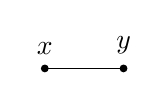
\begin{tikzpicture}
            \node [vertex, label = above:$x$] (x) at (0, 0) {};
            \node [vertex, label = above:$y$] (y) at (1, 0) {};
            \draw (0, 0) -- (1, 0);
        \end{tikzpicture}
        = D_F(x - y);
        \qquad 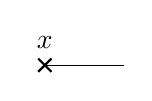
\begin{tikzpicture}
            \node [cross vertex, label = above:$x$] (x) at (0, 0) {};
            \draw (0, 0) -- (1, 0);
        \end{tikzpicture}
        = ij(x),
    \end{equation*}
    and integrating over all internal points. Then $\lambda$ can be represented as
    \begin{equation*}
        \lambda = \int \dd^4x \int \dd^4y \, j(x)D_F(x - y)j(y) = 
        -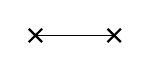
\begin{tikzpicture}
            \node [cross vertex] (x) at (0, 0) {};
            \node [cross vertex] (y) at (1, 0) {};
            \draw (0, 0) -- (1, 0);
        \end{tikzpicture}.
    \end{equation*}
    As we can see, $M$ is the sum of all diagrams without external vertices. Since only diagrams with an even
    number of vertices can be fully connected to yield a non-zero term, we now consider $2n$-th diagram in the 
    perturbation series. It is given by
    \begin{equation*}
        \frac{1}{(2n)!} S \left(
            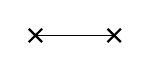
\begin{tikzpicture}
                \node [cross vertex] (x) at (0, 0) {};
                \node [cross vertex] (y) at (1, 0) {};
                \draw (0, 0) -- (1, 0);
            \end{tikzpicture}    
        \right)^n
        = \frac{(-\lambda)^n}{(2n)!} S,
    \end{equation*}
    where $S$ is the number of ways these vertices could be connected. We'll find it in this way: first choose 2 
    vertices from $2n$ vertices to connect, then choose 2 more from the rest $2n - 2$ vertices, and so on, and 
    divide the final result by $n!$ to cancel the order of our steps. Thus
    \begin{equation*}
        S = \frac{1}{n!} C_{2n}^2 C_{2n - 2}^2 \cdots C_2^2
        = \frac{1}{n!} \frac{(2n)!}{2(2n - 2)!} \frac{(2n - 2)!}{2(2n - 4)!}
        \cdots \frac{2!}{2(0!)}
        = \frac{(2n)!}{2^n n!}.
    \end{equation*}
    Substitute into the expression of $2n$-th term, the $(2n)!$ cancels, resulting in another taylor series
    of exponentiate:
    \begin{equation*}
        M = \frac{1}{n!}(-\frac{\lambda}{2})^n = e^{- \lambda / 2}.
    \end{equation*}
    So that $P(0) = \abs{M}^2 = e^{-\lambda}$.

    \item In this case, the initial and final state are
    \begin{equation*}
        \ket{i} = \ket{0}, \qquad \text{and} \quad \ket{f} = a_k^\dagger\ket{0} = \frac{1}{\sqrt{2\omega_k}}\ket{k},
    \end{equation*}
    respectively. The probability is now
    \begin{equation*}
        P(1, k) \equiv \abs{M_k}^2 = \abs{
            \bra{f} T\left\{
                \exp[i\int \dd^4x \, j(x)\phi_I(x)]    
            \right\} \ket{0}
        }^2.
    \end{equation*}
    When expanding, we need the contraction of $\phi_I$ with $\ket{f}$:
    \begin{equation*}
        \wick{\c \phi_I(x) |\c f\rangle}
        = \wick{\c \phi_I(x) \c a_k^\dagger}\ket{0}
        = \sum_{k'} \varphi_{k'} a_{k'} a_k^\dagger \ket{0}
        = \varphi_k \ket{0}
        = \frac{1}{\sqrt{2V\omega_k}} e^{-ik\cdot x}\ket{0}.
    \end{equation*}
    This yields the following rule for external lines:
    \begin{align*}
        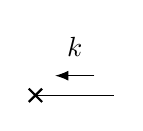
\begin{tikzpicture}[scale = 0.5]
            \node [cross vertex] at (0, 0) {};
            \node [label = above:$k$] at (1, 0.5) {};
            \draw (0, 0) -- (2, 0);
            \draw [-Latex] (1.5, 0.5) -- (0.5, 0.5);
        \end{tikzpicture}
        = i\int \dd^4 x \, j(x) \wick{\c\phi_I(x) \c a_k^\dagger}
        = \frac{i\tilde{\jmath}(k)}{\sqrt{2V\omega_k}}
        \equiv i\mu_k.
    \end{align*}
    Since the final state must contract with one field operator to form a vacuum state, every diagram should contain 
    one vertex that connected to an external line. Thus only $(2n + 1)$-th order 
    diagrams are non-zero, for $n \geqslant 0$. They are given by
    \begin{equation*}
        \frac{1}{(2n + 1)!} S_1 \Big(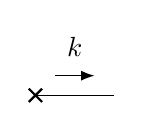
\begin{tikzpicture}[scale = 0.5]
            \node [cross vertex] at (0, 0) {};
            \node [label = above:$k$] at (1, 0.5) {};
            \draw (0, 0) -- (2, 0);
            \draw [-Latex] (0.5, 0.5) -- (1.5, 0.5);
        \end{tikzpicture}\Big) \left(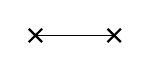
\begin{tikzpicture}
            \node [cross vertex] at (0, 0) {};
            \node [cross vertex] at (1, 0) {};
            \draw (0, 0) -- (1, 0);
        \end{tikzpicture}\right)^n
        = \frac{i}{(2n + 1)!} S_1 \mu_k^\ast (-\lambda)^n,
    \end{equation*}
    where $S_1$, again, is the number of ways these vertices can be connected, can be calculated as
    \begin{equation*}
        S_1 = A_{2n + 1}^1 S = \frac{(2n + 1)(2n)!}{2^nn!}. 
    \end{equation*}
    The diagram then becomes
    \begin{equation*}
        \frac{i}{n!} \left(-\frac{\lambda}{2}\right)^n \mu_k^\ast.
    \end{equation*}
    Thus
    \begin{equation*}
        P(1, k) = \abs{
            i\mu_k^\ast \sum_{n = 0}^\infty
            \frac{1}{n!}
            \left(-\frac{\lambda}{2}\right)^n
        }^2 = \abs{\mu_k}^2 e^{-\lambda}
        = \frac{\abs{\tilde{\jmath}(k)}^2}{2V\omega_k} e^{-\lambda}.
    \end{equation*}

    \item Consider first, the probability of creating $n$ particles with momenta $k_1, k_2, \cdots, k_n$, respectively. The final state is
    \begin{equation*}
        \ket{f} = \prod_{i = 1}^n a_{k_i}^\dagger \ket{0},
    \end{equation*}
    Now $M$ should be the sum of all diagrams with $n$ vertices connected to $n$ different external lines, so only $(2j + n)$-th order diagrams are non-zero:
    \begin{equation*}
        \frac{1}{(2j + n)!} S_n \Big(\prod_{l = 1}^n 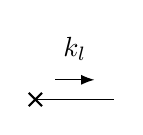
\begin{tikzpicture}[scale = 0.5]
            \node [cross vertex] at (0, 0) {};
            \node [label = above:$k_l$] at (1, 0.5) {};
            \draw (0, 0) -- (2, 0);
            \draw [-Latex] (0.5, 0.5) -- (1.5, 0.5);
        \end{tikzpicture}\Big) \left(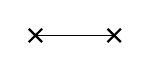
\begin{tikzpicture}
            \node [cross vertex] at (0, 0) {};
            \node [cross vertex] at (1, 0) {};
            \draw (0, 0) -- (1, 0);
        \end{tikzpicture}\right)^j
        = \frac{1}{(2j + n)!} S_n \left(\prod_{l = 1}^n i\mu_{k_l}^\ast\right) (-\lambda)^j.
    \end{equation*}
    Where $S_n$ is the number of contraction ways:
    \begin{equation*}
        S_n = A_{2j + n}^n S 
        = \frac{(2j + n)!}{(2j)!} \frac{(2j)!}{2^jj!} 
        = \frac{(2j + n)!}{2^j j!}.
    \end{equation*}
    Thus
    \begin{equation*}
        M = 
        \left(\prod_{l = 1}^n i\mu_{k_l}^\ast\right) 
        \sum_{j = 0}^\infty 
        j! \left(-\frac{\lambda}{2}\right)^j
        = \left(\prod_{l = 1}^n i\mu_{k_l}^\ast\right)
        e^{-\lambda / 2}.
    \end{equation*}
    The probability of creating $n$ particles is then $\abs{M}^2$ sum over the $n$ momenta, and divide by $n!$
    to cancel the overcounting when interchange these momenta:
    \begin{align*}
        P(n) = \frac{1}{n!}\sum_{\{k_i\}} \abs{M}^2 
        & = \left(
            \sum_k
            \frac{\abs{\tilde{\jmath}(k)}^2}{2V\omega_k}
        \right)^n
        \frac{1}{n!} e^{-\lambda}\\
        & = \left(
            \int \frac{\dd^3k}{(2\pi)^3} \frac{\abs{\tilde{\jmath}(k)}^2}{2\omega_k}    
        \right)^n \frac{1}{n!} e^{-\lambda}\\
        & = \frac{\lambda^n}{n!} e^{-\lambda}.
    \end{align*}

    \item \begin{equation*}
        \sum_{n = 0}^\infty P(n) 
        = e^{-\lambda} \sum_{n = 0}^\infty \frac{\lambda^n}{n!}
        = e^{-\lambda} e^{\lambda} = 1.
    \end{equation*}
    \begin{equation*}
        \avg{N} = \sum_{n = 0}^\infty nP(n)
        = e^{-\lambda} \sum_{n = 1}^\infty \frac{\lambda^n}{(n - 1)!}
        = \lambda e^{-\lambda} \sum_{n = 0}^\infty \frac{\lambda^n}{n!}
        = \lambda.
    \end{equation*}
    \begin{align*}
        \avg{(N - \avg{N})^2} = \avg{N^2} - \avg{N}^2
        & = \avg{N(N - 1)} + \avg{N} - \avg{N}^2\\
        & = e^{-\lambda} \sum_{n = 2}^\infty \frac{\lambda^n}{(n - 2)!}
        + \lambda - \lambda^2\\
        & = \lambda.
    \end{align*}
\end{problembody}

\problem \textbf{Decay of a scalar particle.} Consider the following Lagrangian, involving two
real scalar fiels $\Phi$ and $\phi$:
\begin{equation*}
    \lag = \frac{1}{2}(\partial_\mu\Phi)^2 - \frac{1}{2}M^2\Phi^2
    + \frac{1}{2}(\partial_\mu\phi)^2 - \frac{1}{2}m^2\phi^2
    - \mu\Phi\phi\phi.
\end{equation*}
The last term is an interaction that allows a $\Phi$ particle to decay into two $\phi$'s, provided
that $M > 2m$. Assume that this condition is met, calculate the lifetime of the $\Phi$ to lowest order
in $\mu$.

\solution 
Feynman rule for this Lagrangian is
\begin{equation*}
    \begin{tikzpicture}[baseline = (o)]
        \node [label = above:$k$] (o) at (0, 0) {};
        \draw (-1, 0) -- (1, 0) [arrowed];
    \end{tikzpicture} = \frac{i}{k^2 - m^2 + i\epsilon},
    \qquad 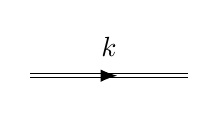
\begin{tikzpicture}[baseline = (o)]
        \node [label = above:$k$] (o) at (0, 0) {};
        \draw [double line] (-1, 0) -- (1, 0) [arrowed];
    \end{tikzpicture} = \frac{i}{k^2 - M^2 + i\epsilon},
\end{equation*}
\begin{equation*}
    \begin{tikzpicture}[baseline = (o.south)]
        \coordinate (a) at (-1, 0);
        \coordinate (b) at (60:1);
        \coordinate (c) at (-60:1);
        \draw [double line] (a) -- (0, 0);
        \draw (b) -- (0, 0) -- (c);
        \node [vertex] (o) at (0, 0) {};
    \end{tikzpicture} = i\mu.
\end{equation*}
The lowest order contribution to the decay of $\Phi$ is given by the tree diagram:
\begin{center}
    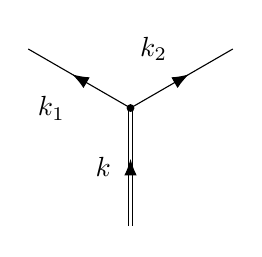
\begin{tikzpicture}[scale = 1.5]
        \coordinate (a) at (0, -1);
        \coordinate (b) at (30:1);
        \coordinate (c) at (150:1);
        \draw [double line] (a) -- (0, 0)[arrowed, text = $k$];
        \draw (0, 0) -- (b) [arrowed, text = $k_2$];
        \draw (0, 0) -- (c) [arrowed, text = $k_1$];
        \node [vertex] at (0, 0) {};
    \end{tikzpicture}.
\end{center}
Thus $i\ims = i\mu$, and the decay width
\begin{align*}
    \dd \Gamma & = \frac{1}{2M(2\pi)^2} 
    \int \dd^3k_1 \int \dd^3k_2 \, \frac{\abs{\ims}^2}{4E_1E_2} \delta(E_1 + E_2 - 2M)\delta^3(k_1 + k_2)\\
    & = \frac{1}{64\pi^2M} \int \dd\Omega 
    \int_0^{+\infty} k^2\dd k \frac{\abs{\ims}^2}{k^2 + m^2}\delta(\sqrt{k^2 + m^2} - M)\\
    %
    & = \frac{\mu^2}{64\pi^2M} \sqrt{1 - \frac{m^2}{M^2}}.
\end{align*}

\problem \textbf{Linear sigma model.} The interactions of pions at low energy can be described
by a phenomenological model called the \textit{linear sigma model}. Essentially, this model 
consists of $N$ real scalar fields coupled by a $\phi^4$ interaction that is symmetric under 
rotations of the $N$ fields. More specifically, let $\Phi^i(x)$, $i = 1, \cdots, N$ be a set of 
$N$ fields, governed by the Hamitonian
\begin{equation*}
    H = \int \dd^3x \, \left(
        \frac{1}{2}(\Pi^i)^2 + \frac{1}{2}(\nabla\Phi^i)^2 + V(\Phi^2)    
    \right),
\end{equation*}
where $(\Phi^i)^2 = \Phi\cdot\Phi$, and
\begin{equation*}
    V(\Phi^2) = \frac{1}{2}m^2(\Phi^i)^2 
    + \frac{\lambda}{4}\left((\Phi^i)^2\right)^2
\end{equation*}
is a function symmetric under rotations of $\Phi$. For (classical) field configurations of $\Phi^i(x)$
that are constant in space and time, this term gives the only contribution to $H$; hence, $V$ is the field
potential energy.

(What does this Hamitonian have to do with the strong interactions? There are two types of light quarks, 
$u$ and $d$. These quarks have identical strong interactions, but different masses. If these quarks are
massless. If these quarks are massless, the Hamitonian of the strong interactions is invariant to unitary
transformations of the 2-component object $(u, d)$:
\begin{equation*}
    \begin{pmatrix}
        u \\ d
    \end{pmatrix} \to \exp(i\vec{\alpha}\cdot\vec{\sigma} / 2)
    \begin{pmatrix}
        u \\ d
    \end{pmatrix}.
\end{equation*}
This is transformation is called an \textit{isospin} rotation. If, in addition, the strong interactions 
are described by a vector ``gluon'' field (as is true in QCD), the strong interaction Hamitonian is invariant
to the isospin rotations done separately on the left-handed and right handed components of the quark fields.
Thus, the complete symmetry of QCD with two massless quarks is $SU(2)\times SU(2)$. It happens that $SO(4)$,
the group of rotations in 4 dimensions, is isomorphic to $SU(2)\times SU(2)$
\footnote{I wonder if this is a mistake, or expressed wrongly, since $SO(4)$ is not a direct product of Lie groups.}, 
so for $N = 4$, the linear 
sigma model has the same symmetry group as the strong interactions.)
\begin{problembody}
    \item Analyze the linear sigma model for $m^2 > 0$ by noticing that, for $\lambda = 0$, the Hamitonian
    given above is exactly $N$ copies of the Klein-Gordon Hamitonian. We can the calculate scattering amplitudes
    as perturbation series in the parameter $\lambda$. Show that the propagator is
    \begin{equation*}
        \wick{\c \Phi^i(x) \c \Phi^j(y)} = \delta^{ij}D_F(x - y),
    \end{equation*}
    where $D_F$ is the standard Klein-Gordon propagator for mass $m$, and that there is one type of vertex gien 
    by
    \begin{equation*}
        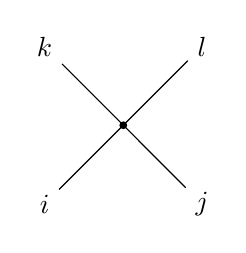
\begin{tikzpicture}[baseline = (o.south)]
            \node (k) at (-1,  1) {$k$};
            \node (l) at ( 1,  1) {$l$};
            \node (i) at (-1, -1) {$i$};
            \node (j) at ( 1, -1) {$j$};
            \draw (k) -- (0, 0) -- (l);
            \draw (i) -- (0, 0) -- (j);
            \node (o) [vertex] at (0, 0) {};
        \end{tikzpicture}
        = -2i\lambda(
            \delta^{ij}\delta^{kl}
            + \delta^{il}\delta^{jk}
            + \delta^{ik}\delta^{jl}
        ).
    \end{equation*}
    (That is, the vertex between two $\Phi^1$s and two $\Phi^2$s has the value $(-2i\lambda)$; that between four 
    $\Phi^1$s has the value $(-6i\lambda)$.) Compute, to leading order in $\lambda$, the differential cross sections 
    $\dd\sigma / \dd\Omega$, in the center of mass frame, for the scattering processes
    \begin{equation*}
        \Phi^1\Phi^2 \to \Phi^1\Phi^2, 
        \qquad \Phi^1\Phi^1 \to \Phi^2\Phi^2,
        \qquad \text{and} \qquad
        \Phi^1\Phi^1 \to \Phi^1\Phi^1
    \end{equation*}
    as functions of the center-of-mass energy.

    \item Now consider the case $m^2 < 0$: $m^2 = -\mu^2$. In this case, $V$ has a local maximum, rather than a minimum,
    at $\Phi^i = 0$. Since $V$ is a potential energy, this implies that the ground state of the theory is not near $\Phi^i = 0$
    but rather is obtained by shifting $\Phi^i$ toward the minimum of $V$. By rotational invariance, we can consider this 
    shift to be in the $N$th direction. Write, then,
    \begin{align*}
        \Phi^i(x) & = \pi^i(x), \qquad i = 1, \cdots, N - 1,\\
        \Phi^N(x) & = v + \sigma(x),
    \end{align*}
    where $v$ is a constant chosen to minimize $V$. (The notation $\pi^i$ suggests a poin field and should not be confused
    with a canonical momentum.) Show that, in these new coordinates (and substituting for $v$ its expression in terms of $\lambda$
    and $\mu$), we have a theory of a massive $\sigma$ field and $N - 1$ \textit{massless} pion fields, interacting through 
    cubic and quartic potential energy terms which all become small as $\lambda \to 0$. Construct the Feynman rules by assigning
    values to the propagators and vertices:
    \begin{align*}
        \wick{\c \sigma \c \sigma} & = \qquad
        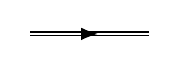
\begin{tikzpicture}[baseline = (o.south)]
            \node (o) [empty]  at (0, 0) {};
            \draw [double line] (0, 0) -- (1.5, 0) [arrowed];
        \end{tikzpicture}
        \qquad\qquad
        \begin{tikzpicture}[baseline = (o.south), scale = 0.6]
            \node (i) at (-150:1.3) {$i$};
            \node (j) at ( -30:1.3) {$j$};
            \draw (-150:1) -- (0, 0) -- (-30:1);
            \draw [double line] (0, 1) -- (0, 0);
            \node (o) [vertex] at (0, 0) {};
        \end{tikzpicture}
        \qquad
        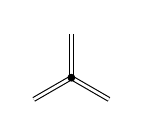
\begin{tikzpicture}[baseline = (o.south), scale = 0.6]
            \node (k) [empty] at (0, 1) {};
            \node (i) [empty] at (-150:1) {};
            \node (j) [empty] at (-30:1) {};
            \draw [double line] (i) -- (0, 0) -- (j);
            \draw [double line] (k) -- (0, 0);
            \node (o) [vertex] at (0, 0) {};
        \end{tikzpicture}\\
        %
        \wick{\c \pi^i \c \pi^j} & = \qquad
        \begin{tikzpicture}[baseline = (i.south)]
            \node (j) [empty, label = right:$j$] at (1.5, 0) {};
            \node (i) [empty, label = left:$i$] at (0, 0) {};
            \draw (0, 0) -- (1.5, 0) [arrowed];
        \end{tikzpicture}
        \qquad\qquad
        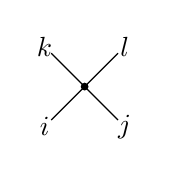
\begin{tikzpicture}[baseline = (o.south), scale = 0.6]
            \node (o) [vertex] at (0, 0) {};
            \draw (135:1) -- (0, 0) -- (45:1);
            \draw (-135:1) -- (0, 0) -- (-45:1);
            \node at (135:1.2) {$k$};
            \node at (45:1.2) {$l$};
            \node at (-135:1.2) {$i$};
            \node at (-45:1.2) {$j$};
        \end{tikzpicture}
        \qquad
        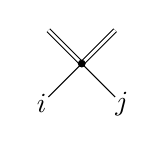
\begin{tikzpicture}[baseline = (o.south), scale = 0.6]
            \draw [double line] (135:1) -- (0, 0) -- (45:1);
            \node (o) [vertex] at (0, 0) {};
            \draw (-135:1) -- (0, 0) -- (-45:1);
            \node at (-135:1.2) {$i$};
            \node at (-45:1.2) {$j$};
        \end{tikzpicture}
        \qquad
        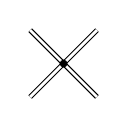
\begin{tikzpicture}[baseline = (o.south), scale = 0.6]
            \draw [double line] (135:1) -- (0, 0) -- (45:1);
            \draw [double line] (-135:1) -- (0, 0) -- (-45:1);
            \node (o) [vertex] at (0, 0) {};
        \end{tikzpicture} 
    \end{align*}

    \item Compute the scattering amplitude for the process
    \begin{equation*}
        \pi^i(p_1)\pi^j(p_2) \to \pi^k(p_3)\pi^l(p_4)
    \end{equation*}
    to leading order in $\lambda$. There are now four Feynman diagrams that contribute:
    \begin{equation*}
        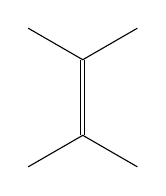
\begin{tikzpicture}[baseline = (o.south), scale = 0.8]
            \coordinate (a) at (0, 0.6);
            \coordinate (b) at (0, -0.6);
            \node (o) [empty] at (0, 0) {};
            \draw [double line] (b) -- (a);
            \draw (a) + (150:1) -- (a) -- +(30:1);
            \draw (b) + (-150:1) -- (b) -- +(-30:1);
        \end{tikzpicture}
        \qquad + \qquad
        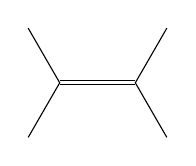
\begin{tikzpicture}[baseline = (o.south), scale = 0.8]
            \coordinate (a) at (0.6, 0);
            \coordinate (b) at (-0.6, 0);
            \node (o) [empty] at (0, 0) {};
            \draw [double line] (b) -- (a);
            \draw (a) + (60:1) -- (a) -- +(-60:1);
            \draw (b) + (120:1) -- (b) -- +(-120:1);
        \end{tikzpicture}
        \qquad + \qquad
        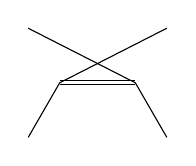
\begin{tikzpicture}[baseline = (o.south), scale = 0.8]
            \coordinate (a) at (0.6, 0);
            \coordinate (b) at (-0.6, 0);
            \node (o) [empty] at (0, 0) {};
            \draw [double line] (b) -- (a);
            \draw (b) + (120:1) -- (a) -- +(-60:1);
            \draw (a) + (60:1) -- (b) -- +(-120:1);
        \end{tikzpicture}
        \qquad + \qquad
        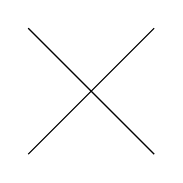
\begin{tikzpicture}[baseline = (o.south), scale = 0.8]
            \node (o) [empty] at (0, 0) {};
            \draw (-1, 1) -- (1, -1);
            \draw (-1, -1) -- (1, 1);
        \end{tikzpicture}
    \end{equation*}
    Show that, at threshold ($\vec{p}_i = 0$), these diagrams sum to \textit{zero}. (Hint: It may be easier to first consider
    the specific process $\pi^1\pi^1 \to \pi^2\pi^2$, for which only the first and fourth diagrams are nonzero, before tackling 
    the general case.) Show that, in the special case $N = 2$ (1 species of pion), the term of $\bigo(p^2)$ also cancels.

    \item Add to $V$ a symmetriy-breaking term,
    \begin{equation*}
        \Delta V = -a\Phi^N,
    \end{equation*}
    where $a$ is a (small) constant. (In QCD, a term of this form is produces if the $u$ and $d$ quarks have the same nonvanishing
    mass.) Find the new value of $v$ that minimizes $V$, and work out the content of the theory about that point. Show that the
    pion acquires a mass such that $m_\pi^2 \sim a$, and show that the pion scattering amplitude at threshold is now nonvanishing
    and also proportional to $a$.
\end{problembody}

\solution
\begin{problembody}
    \item The propagator for this Hamitonian is obvious. Vertex rule can be obtained by considering
    \begin{equation}\label{equ:cp3:vertex_contract}
        \bra{0}T \left[ \Phi^k(x_k)\Phi^l(x_l)\Phi^i(x_i)\Phi^j(x_j) 
            \int \dd^4x \, \frac{-i\lambda}{4} 
            \sum_{m = 1}^N \sum_{n = 1}^N (\Phi^m)^2(\Phi^n)^2
        \right]\ket{0},
    \end{equation}
    and only consider connected part, i.e. the four $\Phi^i$'s outside the integration shouldn't contract with each other. The interchange
    of the $\Phi^m$ and $\Phi^n$ gives a factor of two, while the contraction of the four $\Phi^i$'s with $\Phi^m$ and $\Phi^n$ gives 2, 
    respectively. Thus \eqref{equ:cp3:vertex_contract} becomes
    \begin{equation*}
        -2i\lambda \left(
            \delta^{ij}\delta^{kl} 
            + \delta^{ik}\delta^{jl}
            + \delta^{il}\delta^{jk}    
        \right)
        \int \dd^4x \, D_F(x_k - x)D_F(x_l - x)D_F(x_i - x)D_F(x_j - x).
    \end{equation*}
    So that the vertex rule is given by
    \begin{equation*}
        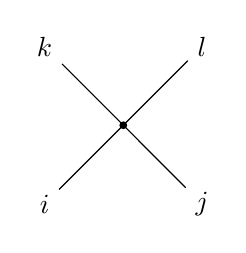
\begin{tikzpicture}[baseline = (o.south)]
            \node (k) at (-1,  1) {$k$};
            \node (l) at ( 1,  1) {$l$};
            \node (i) at (-1, -1) {$i$};
            \node (j) at ( 1, -1) {$j$};
            \draw (k) -- (0, 0) -- (l);
            \draw (i) -- (0, 0) -- (j);
            \node (o) [vertex] at (0, 0) {};
        \end{tikzpicture}
        = -2i\lambda(
            \delta^{ij}\delta^{kl}
            + \delta^{il}\delta^{jk}
            + \delta^{ik}\delta^{jl}
        ).
    \end{equation*}
    Thus
    \begin{equation*}
        i\ims(\Phi^i\Phi^j \to \Phi^k\Phi^l) = -2i\lambda \left(
            \delta^{ij}\delta^{kl}
            + \delta^{il}\delta^{jk}
            + \delta^{ik}\delta^{jl}
        \right) \equiv -2i\lambda A,
    \end{equation*}
    and the cross section
    \begin{equation*}
        \df{\sigma}{\Omega}(\Phi^i\Phi^j \to \Phi^k\Phi^l)
        = \frac{\abs{\ims}^2}{64\pi^2 E_{CM}^2}
        = \frac{\lambda^2 A^2}{16 \pi^2 E_{CM}^2}.
    \end{equation*}
    For the three processes in concern, we have $A = 1, 1, 3$ respectively. As we can see, all of them are isotropic.

    \item In this case, $V$ is given by
    \begin{equation*}
        V = -\frac{1}{2}\mu^2 (\Phi^i)^2 + \frac{\lambda}{4}\left((\Phi^i)^2\right)^2,
    \end{equation*}
    which is quadratic in $(\Phi^i)^2$, and has minimum at $(\Phi^i)^2 = \mu^2 / \lambda$. Thus $v = \mu / \sqrt{\lambda}$. Then
    $V$ becomes
    \begin{align*}
        V & = \frac{\lambda}{4} \left[ (\pi^i)^2 + (v + \sigma)^2\right]^2
        - \frac{1}{2}\mu^2 \left[ (\pi^i)^2 + (v + \sigma)^2 \right]\\
        %
        & = \frac{\lambda}{4}\left((\pi^i)^2\right)^2 + \frac{\lambda}{4}\sigma^4 
        + \sqrt{\lambda} \mu (\pi^i)^2\sigma 
        + \frac{\lambda}{2}(\pi^i)^2\sigma^2
        + \sqrt{\lambda}\mu \sigma^3
        + \mu^2\sigma^2
        - \frac{\mu^4}{4\lambda}.
    \end{align*}
    There is no $(\pi^i)^2$ term, so the $\pi^i$'s are massless, while the term $\mu^2\sigma^2$ indicates $\sigma$ field has mass $\sqrt{2}\mu$, thus the 
    propagators are
    \begin{equation*}
        \wick{\c \pi^i \c \pi^j} = \frac{i\delta^{ij}}{k^2 + i\epsilon}, \qquad
        \wick{\c \sigma \c \sigma} = \frac{i}{k^2 - 2\mu^2 + i\epsilon}.
    \end{equation*}
    Feynman rule can be read directly from $V$:
    \begin{equation*}
        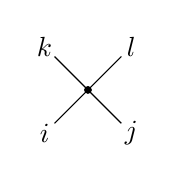
\begin{tikzpicture}[baseline = (o.south), scale = 0.6]
            \draw (135:1) -- (0, 0) -- (45:1);
            \draw (-135:1) -- (0, 0) -- (-45:1);
            \node at (135:1.3) {$k$};
            \node at (45:1.3) {$l$};
            \node at (-135:1.3) {$i$};
            \node at (-45:1.3) {$j$};
            \node (o) [vertex] at (0, 0) {};
        \end{tikzpicture}
        = -2i\lambda\left(
            \delta^{kl}\delta^{ij}
            + \delta^{ki}\delta^{lj}
            + \delta^{kj}\delta^{li}    
        \right),
        \qquad
        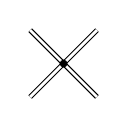
\begin{tikzpicture}[baseline = (o.south), scale = 0.6]
            \draw [double line] (135:1) -- (0, 0) -- (45:1);
            \draw [double line] (-135:1) -- (0, 0) -- (-45:1);
            \node (o) [vertex] at (0, 0) {};
        \end{tikzpicture} = -6i\lambda,
    \end{equation*}
    \begin{equation*}
        \begin{tikzpicture}[baseline = (o.south), scale = 0.6]
            \draw [double line] (0, 0) -- (0, 1);
            \draw (0, 0) -- (-150:1);
            \draw (0, 0) -- (-30:1);
            \node at (-150:1.3) {$i$};
            \node at (-30:1.3) {$j$};
            \node (o) [vertex] at (0, 0){};
        \end{tikzpicture} = -2i\sqrt{\lambda}\mu \delta^{ij},
        \qquad
        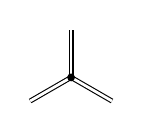
\begin{tikzpicture}[baseline = (o.south), scale = 0.6]
            \draw [double line] (0, 0) -- (0, 1);
            \draw [double line] (-30:1) -- (0, 0) -- (-150:1);
            \node (o) [vertex] at (0, 0){};
        \end{tikzpicture} = -6i\sqrt{\lambda}\mu,
        \qquad
        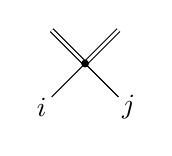
\begin{tikzpicture}[baseline = (o.south), scale = 0.6]
            \draw [double line] (135:1) -- (0, 0) -- (45:1);
            \draw (-135:1) -- (0, 0) -- (-45:1);
            \node at (-135:1.3) {$i$};
            \node at (-45:1.3) {$j$};
            \node (o) [vertex] at (0, 0) {};
        \end{tikzpicture} = -2i\lambda\delta^{ij}.
    \end{equation*}

    \item We evaluate each diagram:
    \begin{align*}
        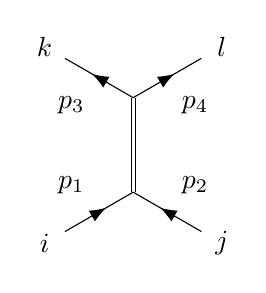
\begin{tikzpicture}[baseline = (o.south)]
            \coordinate (a) at (0, 0.6);
            \coordinate (b) at (0, -0.6);
            \node (o) [empty] at (0, 0) {};
            \draw [double line] (b) -- (a);
            \draw (a) -- +(150:1) [arrowed, text = $p_3$];
            \draw (a) -- +(30:1) [arrowed, texti = $p_4$];
            \node at ($ (a) + (150:1.3) $) {$k$};
            \node at ($ (a) + (30:1.3) $) {$l$};
            \draw ($ (b) + (-150:1) $) -- (b) [arrowed, text = $p_1$];
            \draw ($ (b) + (-30:1) $) -- (b) [arrowed, texti = $p_2$];
            \node at ($ (b) + (-150:1.3) $) {$i$};
            \node at ($ (b) + (-30:1.3) $) {$j$};
        \end{tikzpicture}
        & = -4\lambda\mu^2\delta^{ij}\delta^{kl}\frac{i}{(p_1 + p_2)^2 - 2\mu^2},\\
        %
        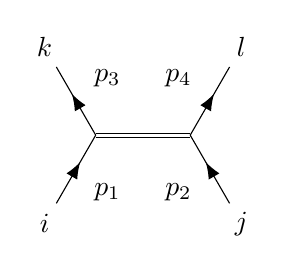
\begin{tikzpicture}[baseline = (o.south)]
            \coordinate (a) at (-0.6, 0);
            \coordinate (b) at (0.6, 0);
            \node (o) [empty] at (0, 0) {};
            \draw [double line] (b) -- (a);
            \draw (a) -- +(120:1) [arrowed, texti = $p_3$];
            \draw (b) -- +(60:1) [arrowed, text = $p_4$];
            \node at ($ (a) + (120:1.3) $) {$k$};
            \node at ($ (b) + (60:1.3) $) {$l$};
            \draw ($ (a) + (-120:1) $) -- (a) [arrowed, texti = $p_1$];
            \draw ($ (b) + (-60:1) $) -- (b) [arrowed, text = $p_2$];
            \node at ($ (a) + (-120:1.3) $) {$i$};
            \node at ($ (b) + (-60:1.3) $) {$j$};
        \end{tikzpicture}
        & = -4\lambda\mu^2\delta^{ki}\delta^{lj}\frac{i}{(p_3 - p_1)^2 - 2\mu^2},\\
        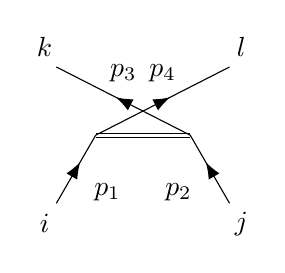
\begin{tikzpicture}[baseline = (o.south)]
            \coordinate (a) at (-0.6, 0);
            \coordinate (b) at (0.6, 0);
            \node (o) [empty] at (0, 0) {};
            \draw [double line] (a) -- (b);
            \draw (a) -- node[midway, label=above:$p_4$] {} ($ (b) + (60:1) $) [arrowed];
            \draw (b) -- node[midway, label=above:$p_3$] {} ($ (a) + (120:1) $) [arrowed];
            \node at ($ (a) + (120:1.3) $) {$k$};
            \node at ($ (b) + (60:1.3) $) {$l$};
            \draw ($ (a) + (-120:1) $) -- (a) [arrowed, texti = $p_1$];
            \draw ($ (b) + (-60:1) $) -- (b) [arrowed, text = $p_2$];
            \node at ($ (a) + (-120:1.3) $) {$i$};
            \node at ($ (b) + (-60:1.3) $) {$j$}; 
        \end{tikzpicture}
        & = -4\lambda\mu^2\delta^{li}\delta^{kj}\frac{i}{(p_4 - p_1)^2 - 2\mu^2},\\
        \begin{tikzpicture}[baseline = (o.south)]
            \draw (135:1) -- (0, 0) -- (-45:1);
            \draw (45:1) -- (0, 0) -- (-135:1);
            \node (o) [empty] at (0, 0) {};
            \node at (135:1.3) {$k$};
            \node at (45:1.3) {$l$};
            \node at (-45:1.3) {$j$};
            \node at (-135:1.3) {$i$};
        \end{tikzpicture}
        & = -2i\lambda\left(
            \delta^{kl}\delta^{ij}
            + \delta^{ki}\delta^{lj}
            + \delta^{kj}\delta^{li}    
        \right).
    \end{align*}
    The amplitude is the sum of the above diagrams:
    \begin{equation*}
        i\ims = -2i\lambda\delta^{ij}\delta^{kl}\frac{s}{s - 2\mu^2}
        - 2i\lambda\delta^{ik}\delta^{lj}\frac{t}{t - 2\mu^2}
        - 2i\lambda\delta^{il}\delta^{kj}\frac{u}{u - 2\mu^2},
    \end{equation*}
    where 
    \begin{equation*}
        s = (p_1 + p_2)^2, \qquad t = (p_3 - p_1)^2, \qquad u = (p_4 - p_1)^2.
    \end{equation*}
    At threshold where $\vec{p}_i = 0$, we have $s = t = u = 0$, so $\ims$ vanishes. In the special case $N = 2$, all
    the $\delta$'s in $\ims$ become factors of one:
    \begin{equation*}
        \ims = -2\lambda\left(
            \frac{s}{s - 2\mu^2}
            + \frac{t}{t - 2\mu^2}
            + \frac{u}{u - 2\mu^2}    
        \right).
    \end{equation*}

    \item With the presence of $\Delta V$, $V$ is now
    \begin{equation*}
        V = \frac{\lambda}{4} \left[
            (\pi^i)^2 + (\Phi^N)^2
        \right]^2
        - \frac{1}{2}\mu^2\left[
            (\pi^i)^2 + (\Phi^N)^2    
        \right]
        - a \Phi^N.
    \end{equation*}
    Let $v$ be the value of $\Phi^N$ that minimizes $V$ when $\pi^i = 0$. The condition is
    \begin{equation*}
        \pd{V}{v} = \lambda v^3 - \mu^2 v - a = 0.
    \end{equation*}
    Since $a$ is small, $v$ can be solved by perturbation. Let $v = \mu / \sqrt{\lambda} + xa + o(a)$, with $x$ be a constant to be
    determined. Substitude into the equation above, we get $x = 1 / 2\mu^2$. The new potential is then
    \begin{align*}
        V & = \frac{\lambda}{4}\left[
            (\pi^i)^2 + (v + \sigma)^2    
        \right] - \frac{1}{2}\mu^2 \left[
            (\pi^i)^2 + (v + \sigma)^2
        \right] - a (v + \sigma)\\
        %
        & = \frac{a\sqrt{\lambda}}{2\mu} (\pi^i)^2 
        + \left(\mu^2 + \frac{3a\sqrt{\lambda}}{2\mu}\right)\sigma^2
        + \left(\frac{a\lambda}{2\mu^2} + \sqrt{\lambda}\mu\right)(\pi^i)^2\sigma
        + \left(\frac{a\lambda}{2\mu^2} + \sqrt{\lambda}\mu\right) \sigma^3\\
        & \qquad + \frac{\lambda}{4}\left((\pi^i)^2\right)^2
        + \frac{\lambda}{2}(\pi^i)^2\sigma^2 + \frac{\lambda}{4}\sigma^4
        -\frac{\mu^4}{4\lambda} - \frac{a\mu}{\sqrt{\lambda}} - o(a).
    \end{align*}
    The $\Delta V$ modifies the particle masses, the $\pi^2\sigma$ and $\sigma^3$ vertices. The pion acquires mass $m_\pi^2 = a\sqrt{\lambda} / \mu \propto a$.
    Since the $\pi^4$ vertex is unaffected, while the coeffecient of $\pi^2\sigma$ vertex is added by $a\lambda / 2\mu^2$, the pion scattering amplitude at threshold 
    now no longer vanish:
    \begin{align*}
        i\ims & = -4i\lambda\left(\mu^2 + \frac{\sqrt{\lambda}}{\mu}a\right)\left(
            \frac{\delta^{ij}\delta^{kl}}{s - m_\sigma^2} 
            + \frac{\delta^{ik}\delta^{lj}}{t - m_\sigma^2} 
            + \frac{\delta^{il}\delta^{kj}}{u - m_\sigma^2}
        \right)\\
        & \qquad -2i\lambda\left(
            \delta^{kl}\delta^{ij}
            + \delta^{ki}\delta^{lj}
            + \delta^{kj}\delta^{li}    
        \right)\\
        %
        & = i\ims_0 + 4i\frac{\lambda\sqrt{\lambda}}{\mu}a \left(
            \frac{\delta^{ij}\delta^{kl}}{s - m_\sigma^2} 
            + \frac{\delta^{ik}\delta^{lj}}{t - m_\sigma^2} 
            + \frac{\delta^{il}\delta^{kj}}{u - m_\sigma^2}
        \right),
    \end{align*}
    where $m_\sigma$ is the mass of ``sigmaon'' with the presence of $\Delta V$, and $\ims$ is the original scattering amplitude with the sigmaon mass in the propagator 
    replaced by $m_\sigma$. Thus $\ims$ vanishes at threshold and the remaining terms are proportional to $a$.
\end{problembody}

\problem \textbf{Rutherford scattering.} The cross section for scattering of an electron by the Coulomb field of a nucleus can be computed, to lowest 
order, without quantizing the electromagnetic field. Insteadm treat the field as a given , classical potential $A_\mu(x)$. The interaction Hamitonian
is 
\begin{equation*}
    H_I = \int \dd^3 x \, e\bar{\psi}\gamma^\mu\psi A_\mu,
\end{equation*}
where $\psi(x)$ is the usual quantized Dirac field.
\begin{problembody}
    \item Show that the \textit{T}-matrix element for electron scattering of a localized classical potential is, to lowest order,
    \begin{equation*}
        \bra{p'}iT\ket{p} = -ie\bar{u}(p')\gamma^\mu u(p) \tilde{A}_\mu(p' - p),
    \end{equation*}
    where $\widetilde{A}_\mu(q)$ is the four dimensional Fourier transform of $A_\mu(x)$.

    \item If $A_\mu(x)$ is time independent, its Fourier transform contains a delta function of energy. It is then natural to define
    \begin{equation*}
        \bra{p'}iT\ket{p} \equiv i\ims (2\pi) \delta(E_f - E_i),
    \end{equation*}
    where $E_i$ and $E_f$ are the initial and final energies of the particle, and to adopt a new Feynman rule for computing $\ims$:
    \begin{equation*}
        \feynmandiagram[horizontal = a to b, baseline = (a.base)]{
            i1 -- [fermion] a [dot] -- [fermion] i2,
            b [crossed dot] -- [photon] a
        };
        = -ie\gamma^\mu\widetilde{A}_\mu(\vec{q}),
    \end{equation*}
    where $\widetilde{A}_\mu(\vec{q})$ is the three dimensional Fourier transform of $A_\mu(x)$. Given this definition of $\ims$, show that the cross section 
    for scattering off a time-independent, localized potential is
    \begin{equation*}
        \dd\sigma = \frac{1}{v_i}\frac{1}{2E_i}\frac{\dd^3p_f}{(2\pi)^3}
        \frac{1}{2E_f}\abs{\ims(p_i \to p_f)}^2 (2\pi)\delta(E_f - E_i),
    \end{equation*}
    where $v_i$ is the particle's initial velocity. This formula is a natural modification of (4.79). Integrate over $\abs{p_f}$ to find a simple expression for $\dd\sigma / \dd \Omega$.

    \item Specialize to the case of electron scattering from a Coulomb potential ($A^0 = Ze / 4\pi r$). Working in the nonrelativistic limit, derive the Rutherford formula,
    \begin{equation*}
        \df{\sigma}{\Omega} = \frac{\alpha^2 Z^2}{4m^2v^4\sin^4(\theta / 2)}.
    \end{equation*}
    (With a few calculational tricks from Section 5.1, you will have no difficulty evaluating the general cross section in the relativistic case; see Problem 5.1.)
\end{problembody}

\solution
\begin{problembody}
    \item \begin{align*}
        \bra{p'}iT\ket{p} & = -ie \int \dd^4x \, 
        \wick{\langle\c p'| \c{\bar\psi}\gamma^\mu\c\psi A_\mu(x) |\c p\rangle}\\
        %
        & = -ie \int \dd^4x \, \bar{u}(p')\slashed{A}(x)u(p) e^{ix\cdot(p' - p)}\\
        & = -ie \bar u(p') \gamma^\mu u(p) \widetilde{A}_\mu(p' - p).
    \end{align*}

    \item The cross section can be derived the same way as (4.79), with
    \begin{equation*}
        \ket{\text{in}} = \int \frac{\dd^3p}{(2\pi)^3} \frac{\phi_i(\vec p)e^{-i\vec b \cdot \vec p}}{\sqrt{2E_p}} \ket{p}_{\text{in}}, \qquad \text{and} \; 
        \ket{\text{out}} = \frac{1}{\sqrt{(2\pi)^32E_f}}\ket{p_f}_{\text{out}}
    \end{equation*}
    being the inital and final states instead, where $\phi_i$ have narrow peak at $p_i$. The cross section is the transition probability integrate over
    the `impact parameter' $\vec b$:
    \begin{align*}
        \frac{\dd\sigma}{\dd^3p_f} & = \int \dd^2b \, \abs{\inner{\text{in}}{\text{out}}}^2\\
        & = \int \dd^2 b \int \frac{\dd^3p_1}{(2\pi)^3} 
        \int \frac{\dd^3p_2}{(2\pi)^3}
        \frac{
            \phi_i^\ast(\vec p_1)
            \phi_i(\vec p_2)
            e^{-i\vec b \cdot (\vec p_2 - \vec p_1)}
        }{
            \sqrt{2E_1}\sqrt{2E_2}(2\pi)^3 2E_f
        }(2\pi)^2\abs \ims^2 \delta(E_1 - E_f) \delta(E_2 - E_f)\\
        & = \frac{1}{(2\pi)^5 2E_f}\int \dd^3p_1 \int \dd^3p_2
        \frac{\phi_i^\ast(\vec p_1)\phi_i(\vec p_2)}{2E_1} \abs \ims^2
        \delta(E_1 - E_2)\delta^2(\vec p_{1\bot} - \vec p_{2\bot})\delta(E_1 - E_f)\\
        & = \frac{1}{(2\pi)^5 2E_f}
        \int \dd^3p_1 \int \dd^3p_2
        \frac{\phi_i^\ast(\vec p_1)\phi_i(\vec p_2)}{2E_1 v_1} \abs \ims^2
        \delta^3(\vec p_1 - \vec p_2)\delta(E_1 - E_f)\\
        & = \frac{1}{(2\pi)^5 2E_f}
        \int \dd^3p_1
        \frac{\abs{\phi_i(\vec p_1)}^2}{2E_1 v_1} \abs \ims^2 \delta(E_1 - E_f)\\
        & = \frac{1}{(2\pi)^2 2E_f 2E_i v_i}\abs\ims^2 \delta(E_i - E_f).
    \end{align*}
    Integrate over modulu,
    \begin{align*}
        \df{\sigma}{\Omega} & = \frac{\abs\ims^2}{16\pi^2 \abs{p_i}} 
        \int_0^\infty \frac{p^2}{2E_f}\delta(E_i - E_f) \dd p\\
        & = \frac{\abs\ims^2}{32\pi^2}.
    \end{align*}

    \item The amplitude in the lowest order is
    \[
        i\ims = -ie\bar u(p_f)\gamma^\mu u(p_i)\widetilde A_\mu(\vec p_f - \vec p_i),
    \]
    where $\widetilde{A}_\mu(\vec q)$ can be calculated below
    \begin{align*}
        \widetilde{A}^0(\vec q) & = \int \dd^3x \, \frac{Ze}{4\pi r} e^{-i\vec q\cdot\vec x}\\
        & = \frac{Ze}{2}\int_0^\pi \dd(-\cos\theta)\int_0^\infty r e^{-iqr\cos\theta} \dd r\\
        & = \frac{Ze}{-2iq}\int_0^\infty e^{-\epsilon r}\left(e^{iqr} - e^{-iqr}\right) \dd r\\
        & = \frac{Ze}{q^2 + \epsilon^2},
    \end{align*}
    and the spacial components are zero. The amplitude then reads
    \begin{align*}
        i\ims & = -ie \bar u(p_f)\gamma^0u(p_i) \frac{Ze}{\abs{\vec p_f - \vec p_i}^2}\\
        & = -2im \delta^{ss'} \frac{Ze^2}{\abs{\vec p_f - \vec p_i}^2}\\
        & = \frac{-i\delta^{ss'}Ze^2}{2mv^2\sin^2(\theta / 2)}.
    \end{align*}
    Thus
    \[
        \df{\sigma}{\Omega} = \frac{e^4Z^2}{64\pi^2 m^2 v^4 \sin^4(\theta / 2)}
        = \frac{\alpha^2Z^2}{4m^2 v^4 \sin^4(\theta / 2)}.    
    \]
\end{problembody}

\bibliographystyle{plain}
\bibliography{cite}
\end{document}